%% This is file `elsarticle-template-1-num.tex',
%%
%% Copyright 2009 Elsevier Ltd
%%
%% This file is part of the 'Elsarticle Bundle'.
%% ---------------------------------------------
%%
%% It may be distributed under the conditions of the LaTeX Project Public
%% License, either version 1.2 of this license or (at your option) any
%% later version.  The latest version of this license is in
%%    http://www.latex-project.org/lppl.txt
%% and version 1.2 or later is part of all distributions of LaTeX
%% version 1999/12/01 or later.
%%
%% The list of all files belonging to the 'Elsarticle Bundle' is
%% given in the file `manifest.txt'.
%%
%% Template article for Elsevier's document class `elsarticle'
%% with numbered style bibliographic references
%%
%% $Id: elsarticle-template-1-num.tex 149 2009-10-08 05:01:15Z rishi $
%% $URL: http://lenova.river-valley.com/svn/elsbst/trunk/elsarticle-template-1-num.tex $
%%
\documentclass[preprint]{elsarticle}

\usepackage[outercaption]{sidecap}
\sidecaptionvpos{figure}{c}
\usepackage{subfigure}
\usepackage{graphicx}
\usepackage{tabularx}
\usepackage{rotating}
\usepackage{url}
\usepackage{listings}
\usepackage{float}
\usepackage{multirow}
\usepackage{hyperref}

%\usepackage{caption}
%\captionsetup{belowskip=12pt,aboveskip=4pt}


\lstset{%
  basicstyle=\ttfamily\scriptsize,%
  columns=fullflexible,% 
  numbers=left,%
  numberstyle=\scriptsize,%
  stepnumber=1,%
  language=C,%
  frame=lrbt,%
  xleftmargin=\fboxsep,%
  xrightmargin=-\fboxsep
}%

\interfootnotelinepenalty=10000

\newfloat{Listing}{h}{myc}
%\AtBeginDocument{\numberwithin{Listing}{section}}

%% Use the option review to obtain double line spacing
%% \documentclass[preprint,review,12pt]{elsarticle}

%% Use the options 1p,twocolumn; 3p; 3p,twocolumn; 5p; or 5p,twocolumn
%% for a journal layout:
%% \documentclass[final,1p,times]{elsarticle}
%% \documentclass[final,1p,times,twocolumn]{elsarticle}
%% \documentclass[final,3p,times]{elsarticle}
%% \documentclass[final,3p,times,twocolumn]{elsarticle}
%% \documentclass[final,5p,times]{elsarticle}
%% \documentclass[final,5p,times,twocolumn]{elsarticle}

%% if you use PostScript figures in your article
%% use the graphics package for simple commands
%% \usepackage{graphics}
%% or use the graphicx package for more complicated commands
%% \usepackage{graphicx}
%% or use the epsfig package if you prefer to use the old commands
%% \usepackage{epsfig}

%% The amssymb package provides various useful mathematical symbols
\usepackage{amssymb}
%% The amsthm package provides extended theorem environments
%% \usepackage{amsthm}

%% The lineno packages adds line numbers. Start line numbering with
%% \begin{linenumbers}, end it with \end{linenumbers}. Or switch it on
%% for the whole article with \linenumbers after \end{frontmatter}.
%% \usepackage{lineno}

%% natbib.sty is loaded by default. However, natbib options can be
%% provided with \biboptions{...} command. Following options are
%% valid:

%%   round  -  round parentheses are used (default)
%%   square -  square brackets are used   [option]
%%   curly  -  curly braces are used      {option}
%%   angle  -  angle brackets are used    <option>
%%   semicolon  -  multiple citations separated by semi-colon
%%   colon  - same as semicolon, an earlier confusion
%%   comma  -  separated by comma
%%   numbers-  selects numerical citations
%%   super  -  numerical citations as superscripts
%%   sort   -  sorts multiple citations according to order in ref. list
%%   sort&compress   -  like sort, but also compresses numerical citations
%%   compress - compresses without sorting
%%
%% \biboptions{comma,round}

% \biboptions{}
\usepackage{atbegshi}% http://ctan.org/pkg/atbegshi


\journal{Journal of Parallel and Distributed Computing}

\begin{document}

\begin{frontmatter}

%% Title, authors and addresses

%% use the tnoteref command within \title for footnotes;
%% use the tnotetext command for the associated footnote;
%% use the fnref command within \author or \address for footnotes;
%% use the fntext command for the associated footnote;
%% use the corref command within \author for corresponding author footnotes;
%% use the cortext command for the associated footnote;
%% use the ead command for the email address,
%% and the form \ead[url] for the home page:
%%
%% \title{Title\tnoteref{label1}}
%% \tnotetext[label1]{}
%% \author{Name\corref{cor1}\fnref{label2}}
%% \ead{email address}
%% \ead[url]{home page}
%% \fntext[label2]{}
%% \cortext[cor1]{}
%% \address{Address\fnref{label3}}
%% \fntext[label3]{}

\title{Damaris: Addressing Performance Variability in Data Management for Post-Petascale Simulations}

%% use optional labels to link authors explicitly to addresses:
%% \author[label1,label2]{<author name>}
%% \address[label1]{<address>}
%% \address[label2]{<address>}

%% Group authors per affiliation:
\author[ens]{Matthieu Dorier\corref{mycorrespondingauthor}}
\cortext[mycorrespondingauthor]{Corresponding author}
\ead{matthieu.dorier@irisa.fr}
\author[inria]{Gabriel Antoniu}
\author[anl]{Franck Cappello}
\author[anl,uiuc]{Marc Snir}
\author[uiuc]{Roberto Sisneros}
\author[inria]{Or\c{c}un Yildiz}
\author[inria]{Shadi Ibrahim}
\author[anl]{Tom Peterka}
\author[cmich]{Leigh Orf}
%\author[uiuc]{Dave Semeraro}



\address[ens]{ENS Rennes, IRISA, Rennes, France}
\address[inria]{Inria, Rennes - Bretagne Atlantique Research Centre, France}
\address[anl]{Argonne National Laboratory, Lemont, IL, USA}
\address[uiuc]{University of Illinois at Urbana Champaign, IL, USA}
\address[cmich]{Central Michigan University, MI, USA}

\begin{abstract}
%Over the past few years, the increasing gap between the computational performance
%and the performance of I/O systems in post-petascale supercomputers has led to new approaches
%to data management. While some of these approaches focus on improving the I/O
%and storage performance for the immense amounts of data produced by HPC simulations,
%other aim to directly connect analysis and visualization tools to running simulations, bypassing
%data storage in order to retrieve a scientific insight earlier on. An important challenge
%for these new approaches consists of reducing the high performance variability.
With exascale computing on the horizon, reducing performance variability in data management tasks (storage, visualization, analysis, etc.) is becoming a key challenge in sustaining high performance.
This variability significantly impacts the overall application performance at scale and its predictability over time. 

In this paper, we present Damaris, a system that leverages \emph{dedicated cores}
in multicore nodes to offload data management tasks, including I/O, data compression,
scheduling of data movements, in situ analysis and visualization. We evaluate Damaris
with the CM1 atmospheric simulation and the Nek5000 computational fluid dynamic simulation 
on four platforms, including NICS's Kraken and NCSA's Blue Waters.
Our results show in particular that 
(1) Damaris fully hides the I/O variability as well as all I/O-related costs, which 
makes simulation performance predictable; 
(2) it increases the sustained write throughput by a factor of up to 15 compared with standard I/O approaches; 
(3) it allows almost perfect scalability of the simulation up to over 9,000 cores, as opposed to state-of-the-art 
approaches that fail to scale;
(4) it enables a seamless connection to the VisIt visualization software to perform in situ analysis and visualization
in a way that does not impact the performance of the simulation, nor its variability.

In addition, we further extended our implementation of Damaris to also support the use of \emph{dedicated
nodes} and conducted a thorough comparison of the two approaches --dedicated cores and dedicated nodes--
for I/O tasks with the aforementioned applications.
\end{abstract}

\begin{keyword}
Exascale Computing, I/O, In Situ Visualization, Dedicated Cores, Dedicated Nodes, Damaris
\end{keyword}

\end{frontmatter}

%\tableofcontents

%%
%% Start line numbering here if you want
%%
% \linenumbers

%% main text
\section{Introduction}
\label{sec:introduction}
As supercomputers become larger and more complex, one critical challenge is to efficiently handle the immense amounts of data generated by extreme-scale simulations. The traditional approach to data management consists of writing data to a parallel file system, using a high-level I/O library on top of a standardized interface such as MPI-I/O. This data is then read back for analysis and visualization purpose.

One major issue posed by this traditional approach to data management is that it induces a high performance variability. This variability can be observed at different levels. Within a single application, I/O contention across processes leads to large variations in the time each process takes to complete its I/O operations (I/O jitter). Such differences from a process to another in a massively parallel application makes all processes wait for the slowest one. These processes thus waste valuable computation time. The variability is even larger from one I/O phase to another, due to interference with other applications sharing the same parallel file system. 

While scientists have found a potential solution to this problem by coupling their simulations with visualization software in order to bypass data storage and derive results early on, the current practices of coupling simulations with visualization tools also expose simulations to high performance variability, as their run time does not depend anymore on their own scalability only, but also on the scalability of visualization algorithms. This particular problem is further amplified in the context of interactive in situ visualization, where the user himself and his interactions with the simulation become the cause of run-time variability. 

To make an efficient use of future exascale machines, it becomes important to provide data management solutions that do not solely focus on pure performance, but address performance variability as well. Addressing this variability is indeed the key to ensure that each and every component of these future platforms is optimally used.

To address these challenges, we have proposed a new system for I/O and data management called Damaris. Damaris leverages dedicated I/O cores on each multicore SMP (Symmetric multiprocessing) node, along with the use of shared memory, to efficiently perform asynchronous data processing I/O and in situ visualization. We picked this approach based on the intuition that the usage of dedicated cores for I/O-related tasks combined with the usage of intranode shared memory can help overlapping I/O with computation, but also lowering the pressure on the storage system by reducing the number of files to be stored and, at the same time, the amount of data. Such dedicated resources can indeed perform data aggregation, filtering or compression, all in an asynchronous manner. Moreover, such dedicated cores can further be leveraged to enable non-intrusive in situ data visualization with optimized resource usage. Some of these aspects of the Damaris approach have been introduced in previous conference papers~\cite{dorier2012damaris,dorier2013damarisviz}. This paper aims to provide a comprehensive, global presentation and discussion of the Damaris approach in its current state and of its evaluation and applications.

We evaluated Damaris on three different platforms including the Kraken Cray XT5 supercomputer~\cite{kraken}, with the CM1 atmospheric model~\cite{bryan2002benchmark} and the Nek5000~\cite{nek5000} computational fluid dynamics code. By overlapping I/O with computation and by gathering data into large files while avoiding synchronization between cores, our solution brings several benefits: (1) it fully hides the jitter as well as all I/O-related costs, which makes the simulation’s performance predictable; (2) it substantially increases the sustained write throughput (by a factor of 15 in CM1, 4.6 in Nek5000) compared with standard approaches; (3) it allows almost perfect scalability of the  simulation (up to over 9,000 cores with CM1 on Kraken), as opposed to state-of-the-art approaches which fail to scale; (4) it enables data compression without any additional overhead, leading to a major reduction of storage requirements.

Furthermore, we extended Damaris with Damaris/Viz, an in situ visualization framework based on the Damaris approach. By leveraging dedicated cores, external high-level structure descriptions and a simple API, our framework provides adaptable in situ visualization to existing simulations at a low instrumentation cost. Results obtained with the Nek5000 and CM1 simulations show that our framework can completely hide the performance impact of visualization tasks and the resulting run-time variability. In addition, the proposed API allows efficient memory usage through a shared-memory-based, zero-copy communication model.

Finally, in order to compare the Damaris, dedicated-core-based approach with other approaches such as dedicated nodes, forwarding nodes, and staging areas, we further extended Damaris to support the use of dedicated nodes as well. We leverage again the CM1 and Nek5000 simulations on Grid'5000, the national French grid testbed, to shed light on the conditions under which a dedicated-core-based approach to I/O is more suitable than a dedicated-node-based one, and vice versa.

To the best of our knowledge, Damaris is the first open-source middleware to enable the use of dedicated cores or/and dedicated nodes for data management tasks ranging from storage I/O to complex in situ visualization scenarios.

The rest of this paper is organized as follows: Section~\ref{sec:background} presents the background and motivation for our work, discusses the limitations of current approaches to I/O and to in situ visualization. Our Damaris approach, including its design principles, implementation detail and use cases, is described in Section~\ref{sec:damaris}. We evaluate Damaris in Section~\ref{sec:evaluation}, first in scenarios related to storage I/O, then in scenarios related to in situ visualization. Our experimental evaluation continues in Section~\ref{sec:discussion} with a comparison between dedicated cores and dedicated nodes in various situations. Section~\ref{sec:related} discusses our positioning with respect to related work and Section~\ref{sec:conclusion} summarizes our conclusions and discusses open further directions.




\section{Background and Motivation}
\label{sec:background}
HPC simulations create large amounts of data that are then read offline by analysis tools. 
In the following we present the traditional approaches to parallel I/O as well
as the problems they pose in terms of performance variability. We then dive into the trend toward
coupling simulations with analysis and visualization tools, going from offline to in situ analysis and
visualization.

\subsection{I/O and Storage for Large-Scale HPC Simulations}
			
			Two I/O approaches are commonly have been traditionally used for performing I/O in large-scale simulations.
%
			\begin{description}
		
			\item[The File-per-process] approach consists of having each process access its own file.
			This reduces possible interference between the I/O of different processes, but  increases the number of metadata operations. 
			This is especially a problem for file systems with a single metadata server, such as Lustre~\cite{schwan2003lustre}. 
			It is also hard to manage the large number of files thus created and have them read by  analysis or visualization 
			codes that use a different number of processes
			
			\item[Collective I/O] leverages communication phases between
			processes to aggregate access requests and reorganize them. These operations
			are typically used when several processes need to access different parts
			of a shared file, and benefit from tight interactions between the file system
			and the MPI-I/O layer in order to optimize the application's access pattern~\cite{prost2006mpi}.
			
			\end{description}
%
			\subsubsection{Variability in Traditional I/O Approaches}

			The periodic nature of scientific simulations, which alternate between computation and I/O phases,
			leads to burst of I/O activity. The overlap between computation and I/O is reduced, so that both the compute 
			nodes and the I/O subsystem may be idle for periods of time.
		
			With larger machines, the higher degree of I/O concurrency between processes of a single application
			or between concurrent applications pushes the I/O system to its limits. This
			leads to a substantial variability in I/O performance.
			Reducing or hiding this variability is critical, as it is an effective way to make
			a more efficient use of these new computing platforms through improved
			predictability of the behavior and of the execution time of applications.
			
			Figure~\ref{fig:ior:variability} illustrates this variability with the IOR application~\cite{shan2007using},
			a typical benchmark used to evaluate the performance of parallel file systems with pre-defined
			I/O patterns. It shows that even with very well optimized I/O (each process here writes the same amount
			of data contiguously in a separate file using large requests that match the file system's distribution policy) 
			there is a large difference in the time taken by each
			process to complete its I/O operations within a single I/O phase and also across I/O phases.
			Since during these I/O phases all processes have to wait for the slowest one before resuming computation, 
			this I/O variability leads to a waste of performance and to unpredictable overall run times.
			I/O variability is therefore a key issue that we aim to address in this paper.
			
			\begin{figure}
				\begin{center}
				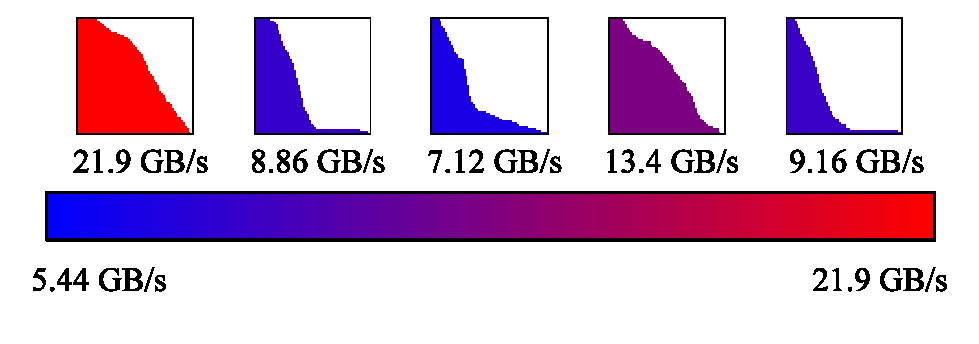
\includegraphics[width=10cm]{figures/variability.eps}
				\caption[somthing]{Variability across processes and across I/O phases in the IOR benchmark using a file-per-process approach
				on Grid'5000's Rennes site~\protect\cite{grid5000}, with a PVFS2~\protect\cite{carns2000pvfs} file system.
				Each graph represents a write phase. The 576 processes are sorted by write time on the $y$ axis and
				an horizontal line is draw with a length proportional to this write time. These graphs are normalized
				so that the longest write time spawns the entire graph. Each graph is colored according to
				a scale that gives the aggregate throughput of the phase, that is, the total amount
				of data written divided by the write time of the slowest process.\footnotemark}\label{fig:ior:variability}
				\end{center}
			\end{figure}
			
			\AtBeginShipoutNext{\footnotetext{Due to the use of colors, this figure may not be properly interpretable if this document
			was printed in black and white. Please refer to an electronic version.}}
			
		\subsubsection{Causes and Effects of the I/O Variability}
		
			Skinner at al.~\cite{skinner2005understanding} point out four causes of 
			performance variability in supercomputers (here presented in a different order).
%
			\begin{enumerate}
			
			\item Communication, causing synchronization between
			processes that run within the same node or on separate nodes. In
			particular, network access contention causes collective
			algorithms to suffer from variability in point-to-point communications.
			
			\item Kernel process scheduling, together with the jitter introduced by
			the operating system.
			
			\item Resource contention within multicore nodes, caused by
			several cores accessing shared caches, main memory and network devices.
			
			\item Cross-application contention, which constitutes a random
			variability coming from simultaneous accesses to shared components of the
			computing platform, such as the network or the storage system, by distinct applications.
		
			\end{enumerate}
%
			Future systems will have additional sources of variability, such as power management, and fault masking activities.
			Issues 1 and 2, respectively, cause communication and computation jitter.
			Issue 1 can be addressed through more efficient network hardware 
			and collective communication algorithms. The use of 
			lightweight kernels with less support for process scheduling can alleviate issue 2. 
			Issues 3 and 4, on the other hand, cause I/O performance variability.
		
			At the level of a node, the increasing number of cores per node in recent machines makes 
			it difficult for all cores to access the network all at once with an optimal 
			throughput. Requests are serialized in network devices, leading to a different service
			time for each core. This problem is further amplified by the fact that an I/O 
			phase consists of many requests that are thus serialized in an unpredictable manner.

			Parallel file systems also represent a well-known bottleneck and a source of high
			variability~\cite{uselton2010parallel}. The time taken
			by a process to write some data can vary by several orders of
			magnitude from one process to another and from one I/O phase to
			another depending on many factors, including (1) network contention 
			when several nodes send requests to the same I/O server~\cite{dorier2014calciom}, 
			(2) access contention at the level of the file system's metadata server(s) 
			when many files are created simultaneously~\cite{dorier:inria-00614597},
			(3) unpredictable parallelization of I/O requests across I/O servers due to different 
			I/O patterns~\cite{lofstead2010managing}, (4) additional disk-head movements due 
			to the interleaving of requests coming from different processes or applications~\cite{gainaru2014scheduling}.
			Other source of I/O variability at disk level include the overheads of RAID group reconstruction, 
			data scrubbing overheads, or various firmware activities.
		
			Lofstead et al.~\cite{lofstead2010managing} present I/O variability in terms
			of \emph{interference}, with the distinction between \emph{internal
			interference} caused by access contention between processes of
			the same application, and \emph{external interference} that are due to
			sharing the access to the file system with other applications,
			possibly running on different clusters.
			While the sources of I/O performance variability are numerous and difficult to track, we can indeed
			observe that some of them originate from contentions within a single application,
			while other come from the contention between multiple applications concurrently running on
			the same platform. The following section describes how to tackle these two sources of contention.
						
		\subsubsection{Approaches to Mitigate the I/O Variability}

			While most efforts today address performance and scalability issues for
			specific types of workloads and software or hardware components, few
			efforts target the causes of performance variability. We highlight two
			practical ways of hiding or mitigating the I/O variability.

			\paragraph{Asynchronous I/O}
				The main solution to prevent an application from being impacted by its I/O consists
				of using asynchronous I/O operations, i.e., non-blocking operations that proceed in
				the background of the computation.
	
				The MPI 2 standard proposes rudimentary asynchronous I/O functions
				that aim to overlap computation with I/O. Yet these functions are available only 
				for independent I/O operations. Besides, popular implementations of the MPI-I/O
				standard such as ROMIO~\cite{thakur1999on} actually implement most of these functions
				as synchronous. Only the small set of functions that handle contiguous accesses have
				been made asynchronous, provided that the backend file system supports it.
	
				Released in 2012, the MPI 3 standard completes this interface with asynchronous 
				collective I/O primitives. Again, their actual implementation is mostly synchronous.
				As of today, there is no way to leverage completely asynchronous I/O using only MPI-I/O.
				Higher-level libraries such as HDF5~\cite{hdf5,folk1999hdf5} or NetCDF \cite{netcdf} 
				have also no support yet for asynchronous I/O.
			
			\paragraph{Dedicated I/O Resources}
				Over the past few years, dedicated I/O resources have been proposed to address the
				limitation of MPI implementations in terms of asynchronous I/O. These resources can take various forms. 
				Explicit I/O threads~\cite{fu2012iothreads} have been used to achieve fully asynchronous
				I/O at the potential price of additional OS jitter.
				Dedicated cores have been proposed to leverage a subset of cores in each multicore node used 
				by the application~\cite{dorier2012damaris,li2010functional}, and have them perform I/O operations on behalf of the
				cores that run the application. Staging areas~\cite{abbasi2009datastager,nisar2009scaling,prabhakar2011provisioning} is another
				approach that usually consists of dedicated nodes deployed along with an application.
				Forwarding nodes~\cite{ali2009scalable,stone2006pdio} and burst buffers~\cite{liu2012role,ma2006highlevel} consist of a set 
				of nodes, independent of the applications and interposed between the compute nodes 
				and the storage system. These nodes may feature a larger memory capacity than compute nodes,
				in the form of SSDs or NVRAMs.
				
				This trend toward using dedicated resources has benefited the field of data
				analysis and visualization as well, where dedicated cores or nodes are seen as new ways to 
				efficiently get access to simulations' data as they are generated. The next section
				explores this trend in more details.
				
\subsection{Analysis and Visualization: an Overlooked Process}

	Data produced by HPC simulations can serve several purposes. 
	One of them is fault tolerance using a checkpoint/restart method.
	The other, and most important, is the analysis and visualization of the simulated phenomenon.
	Analysis and visualization are important components of the process that leads
	from running a simulation to actually \emph{discovering knowledge}.
	
	Given the increasing computation power in recent machines and the trend toward using dedicated resources,
	it will become more and more common to couple the simulation with the analysis and visualization tools.
	Simulation/Visualization coupling consists of making the simulation send its data directly to
	a visualization software instead of storing it and processing it offline.
	This approach, termed \textit{in situ visualization} and illustrated in
	Figure~\ref{fig:simviz} (b), has the advantage of bypassing the 
	storage system and producing results faster. It also allows scientists to control their simulations
	as they run, efficiently overlapping simulation and knowledge discovery.
	
	\begin{figure}
		\begin{center}
		\subfigure[Traditional Scientific Workflow]{
			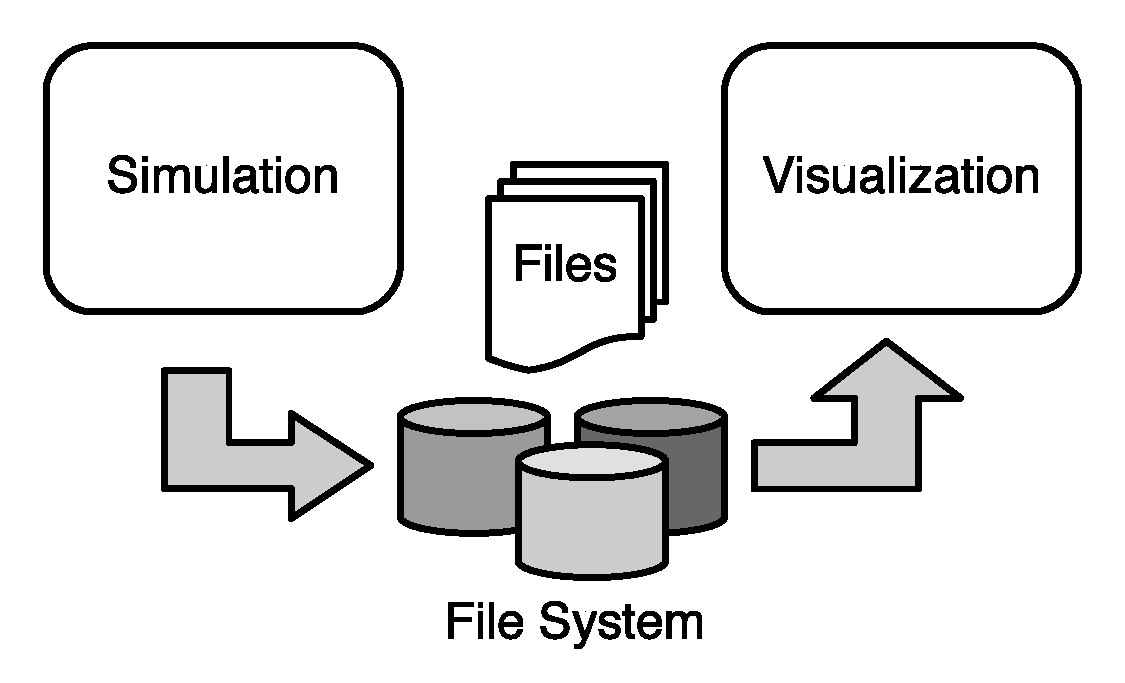
\includegraphics[width=5.5cm]{figures/simviz1.eps}
		}
		\subfigure[Coupling Simulation/Visualization]{
			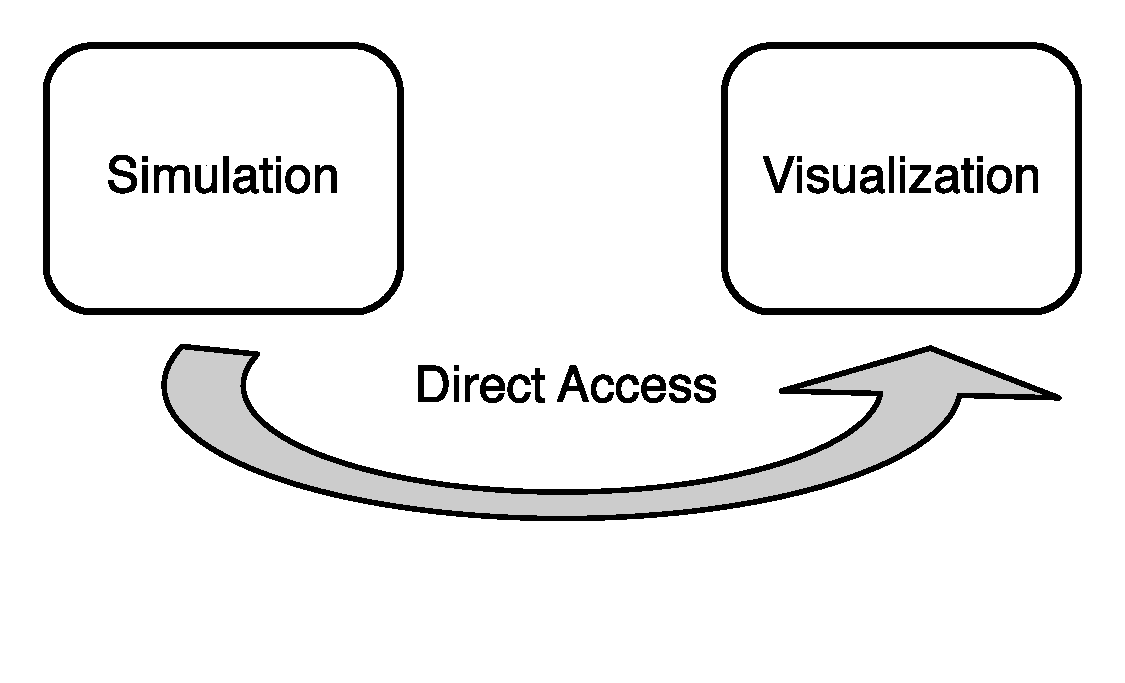
\includegraphics[width=5.5cm]{figures/simviz2.eps}
		}
		\caption{Two approaches to retrieve 
		insight from large-scale simulations: (a) the traditional approach of storing data in a parallel
		file system and reading it offline, (b) the new trend towards simulation/visualization coupling.}\label{fig:simviz}
		\end{center}
	\end{figure}
	
	\subsubsection{A Taxonomy of In Situ Visualization Methods}

	Several in situ visualization strategies exist that we separate into two main categories 
	--tightly coupled and loosely coupled-- depending on where visualization tasks run.

		\paragraph{Tightly-Coupled In Situ Visualization} 
		In a tightly-coupled scenario, the analysis and visualization codes run on the same node 
		as the simulation and share its resources. The main advantage of this scenario is the proximity 
		to the data, which can be retrieved directly from the memory of the simulation. 
		Its drawback lies in the impact that such analysis and visualization tasks can have on the performance 
		of the simulation and on the variability of its run time. Within this category, we make a distinction between
		\emph{time partitioning} and \emph{space partitioning}. 
		
		Time-partitioning visualization consists of periodically stopping the simulation to perform visualization tasks. 
		This is the most commonly used method. For example, it is implemented in VisIt's \emph{libsim}
		library~\cite{whitlock2011parallel} and ParaView's \emph{Catalyst} 
		library~\cite{fabian2011paraview,catalyst}.

		In a space-partitioning mode, dedicated cores perform visualization in parallel with the simulation.
		This mode poses challenges in efficiently sharing data between the cores running the simulation and
		the cores running the visualization tasks, as these tasks progress in parallel. It also
		reduces the number of cores available to the simulation.
		
		\paragraph{Loosely-Coupled In Situ Visualization} 
		In a loosely coupled scenario, analysis and visualization codes run on a separate set of
		resources, that is, a separate set of nodes located either in the same supercomputer as
		the simulation~\cite{zheng2010predata,rasquin2011electronic}, 
		or in a remote cluster~\cite{malakar2010adaptive}. 
		The data is sent from the simulation to the visualization nodes through the network. 
		
		Some in situ visualization frameworks such as GLEAN~\cite{hereld2011toward} can be considered hybrid, placing
		some tasks close to the simulation in a time-partitioning manner while other tasks
		run on dedicated nodes.
	
	\subsubsection{From Offline to In Situ Visualization: Another Source of Variability}
	
		The increasing amounts of data generated by scientific simulations also leads to performance
		degradations when it comes to reading back data for analysis and visualization~\cite{childs2010extreme,yu2005study}.
		While I/O introduces run time variability, in situ analysis and visualization can also negatively impact
		the performance of the simulation/visualization complete workflow. 
		For instance, periodically stopping the simulation to perform in situ visualization in a time-partitioning manner
		leads to a loss of performance and an increase of run-time variability. 
		Contrary to the performance of the simulation itself,
		the performance of visualization tasks may depend on the
		content of the data and is therefore unbalanced across processes and across iterations.
		This variability is further amplified if the in situ visualization framework is interactive, in which case the user
		himself impacts the performance of his application.
	
		In a loosely-coupled approach to in situ visualization, sending data through the network potentially impacts the performance of
		the simulation and forces a reduced number of nodes to sustain the input of a large amount of data.
		Transferring such large amounts of data through the network also have a potentially larger
		impact on the simulation than running visualization tasks in a tightly-coupled manner.
		
\subsection{Our Vision: Using Dedicated Cores for I/O and In Situ Visualization}
	
		Despite the limitations of the traditional, offline approach to data analysis and visualization,
		users  are still seldom moving to purely in situ visualization and analysis~\cite{yu2010insitu,ma2007insitu,ma2009insitu}.
		The first reason is the development cost of such a step in large codes that were maintained for decades.
		The second reason is that storage I/O is still required for checkpoint-based fault tolerance, which makes
		offline analysis of checkpoints the natural candidate for scientific discovery.
			
		To push further the adoption of in situ visualization and increase the productivity of the overall
		scientific workflow, \emph{we postulate that a framework should be provided that deals with
		all aspects of Big Data management in HPC simulations}, including efficient I/O but also
		in situ processing, analysis and visualization of the produced data.
		Such a framework can at the same time provide efficient storage I/O for data that need to be stored,
		and efficient in situ visualization to speed up knowledge discovery and enable simulation monitoring.
		
	%	We postulate that four main requirements will drive the adoption of such a framework.
	%
	%	\begin{description}
		
	%		\item[Low impact on run time:] As explained earlier, using computational resources collocated
	%		with the simulation can affect the performance of the underlying simulation. This is 
	%		especially true when interactive systems directly connect users to their running simulation.
	%		
	%		\item[Optimized resource utilization:] Collocated simulations and
	%		post-processing codes share resources such as local memory and network bandwidth.
	%		Efficiently using these resources is critical for an approach to be suitable at a very large scale.
			
	%		\item[Low impact on the code:] Users are less likely to adopt a new
	%		approach to data management if it requires many code changes in their simulation and the 
	%		understanding of new tools~\cite{thompson2009design}, or if a I/O and visualization
	%		specialist should be consulted for that.
			
	%		\item[High adaptability:] The framework should be adaptable to many simulations and
	%		many data processing scenarios. In particular it should enable to switch visualization
	%		backends or seamlessly leverage a wide range of external data-processing libraries.
		
	%	\end{description}
	%
		Over the past 4 years we have been addressing this challenge by proposing, designing and
		implementing the Damaris system to data management.
		%, within the context of the Joint INRIA-UIUC-ANL
		%Laboratory for Petascale Computing (JLPC). 
		Damaris proposes to dedicate cores
		in multicore nodes for any type of data management task, including I/O and in situ visualization.
		We tried to make Damaris \emph{simple to use}, \emph{flexible}, \emph{portable} and \emph{efficient} 
		in order to ease its adoption by the HPC community. 
		%As a consequence, Damaris was one of the first results of the JLPC to be formally
		%validated for use on the Blue Waters Petascale project~\cite{sisneros2013application}.
		The following section gives an overview of this approach and its implementation.
		


\section{The Damaris Approach: an Overview}
\label{sec:damaris}
In order to address both I/O and in situ analysis/visualization issues,
we propose to gather the I/O operations into a set of dedicated cores in each
multicore node. These cores (typically one per node)
are dedicated to data management tasks (i.e., they do not run the simulation code) in order
to overlap writes and analysis tasks with computation and avoid contention for accesses
to the file system. The cores running the simulation
and the dedicated cores communicate data through shared memory.
We call this approach Damaris. Its design, implementation and API are described below.

\subsection{Design Principles}

The Damaris approach is based on four main design principles.

\subsubsection{Dedicated Cores}

The Damaris approach is based on a set of processes running on dedicated cores in every multicore node.
Each dedicated core performs in situ processing and I/O in response to user-defined events sent by the simulation.
We call a process running the simulation a \emph{client}, and a process running on a dedicated core a \emph{server}.
One important aspect of Damaris is that dedicated cores do not run the simulation.
With the current trend in hardware solutions, the number of cores per node increases.
Thus dedicating one or a few cores has a diminishing impact on the performance of the simulation. 
Hence, our approach primarily targets SMP nodes featuring a large number of cores per node: 12 to 24 in our experiments.

\subsubsection{Data Transfers through Shared Memory}

Damaris handles large data transfers from clients to servers through shared memory.
This makes a write as fast as a \texttt{memcpy} and also enables direct allocation of
variables within the shared memory. This option is especially useful to reduce the
memory requirements of in situ visualization tasks, which can directly access the memory
of the simulation without requiring a copy (see our previous work~\cite{dorier2013damarisviz}).

\subsubsection{High-Level Data Abstraction}

Clients write enriched datasets in a way similar to scientific I/O libraries such as HDF5~\cite{folk1999hdf5} or NetCDF~\cite{netcdf}.
That is, the data output by the simulation is organized into a hierarchy of groups and variables,
with additional metadata such as the description of variables, their type, unit, and layout in memory.
The dedicated cores thus have enough knowledge of incoming datasets to write them in existing high-level 
formats. This design principle differs from other approaches that capture I/O operations at a lower 
level~\cite{li2010functional,ma2006highlevel}. These approaches indeed lose the semantics of the data being written.
While our design choice forces us to modify the simulation so that it writes its data using Damaris' API,
is allows to implement semantic-aware data processing functionalities in dedicated cores. In particular, keeping
this level of semantics is mandatory in order for dedicated cores to be able to write data in a standard, high-level
format such as HDF5 or NetCDF, or to feed an in situ visualization pipeline.

\subsubsection{Extensibility through Plugins}

Servers can perform data transformations prior to writing them, as well as analysis and visualization.
One major design principle in the Damaris approach is the possibility for users to provide these 
transformations through a plugin system, thus adapting Damaris to the particular requirements of 
their application. Implementing such a plugin system at a lower level would
not be possible, as it would not have access to the high-level information about
the data (e.g., dimensions of arrays, data types, physical meaning of the variable 
within the simulation, etc.).

\subsection{Architecture}

\begin{figure}
	\begin{center}
	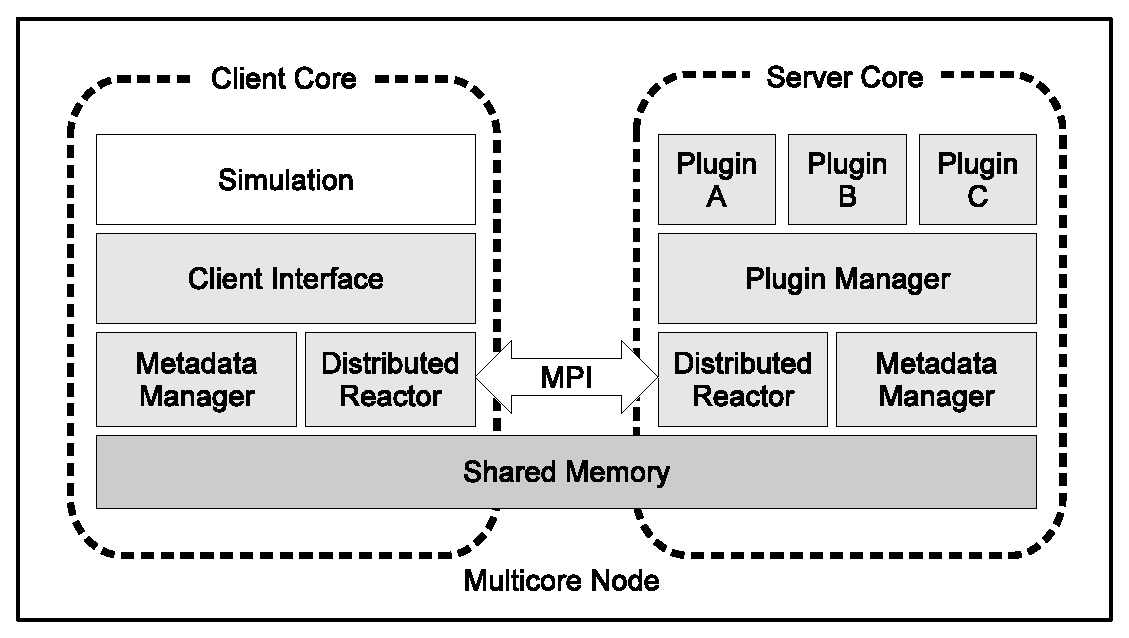
\includegraphics[width=\textwidth]{figures/damaris-schema.eps}
	\caption[Software architecture of the implementation of Damaris]{Software architecture of the implementation of Damaris.}\label{fig:damaris:design}
	\end{center}
\end{figure}

Figure~\ref{fig:damaris:design} presents the software architecture underlying the Damaris approach.
While Damaris can dedicate several cores in large multicore nodes, only one client
and one server are represented here.

Damaris has been designed in a highly modular way and features
a number of decoupled, reusable software components.
The \emph{Shared Memory} component handles the shared buffer and ensures the safety of
concurrent allocations/deallocations. The \emph{Distributed Reactor} handles communications between 
clients and servers, and across servers. The \emph{Metadata Manager} stores high-level information 
related to the data being transferred (type, size, layout, etc.).
Finally the \emph{Plugin Manager} on the server side loads and runs user-provided plugins.

This modular architecture greatly simplified the
adaptation to several HPC platforms and simulations, as well as the development of
extensions to support various scenarios such as storage, in situ visualization, data compression 
or I/O scheduling. The following sections describe each component in more detail.

\subsubsection{Shared Memory}

Data communications between the clients and the servers are
performed through the Shared Memory component. A large
memory buffer is created on each node by the dedicated cores at start time, with a size set by the user 
(typically several MB to several GB). 
Thus the user has full control over the resources allocated to Damaris.
When a client submits new data, it reserves a segment of this shared-memory buffer. 
It then copies its data using the returned pointer so that the local memory can be reused.

\subsubsection{Distributed Reactor}

The Distributed Reactor is the most complex component of Damaris.
It builds on the \emph{Reactor} design pattern~\cite{coplien95reactor} to provide the means 
by which different cores (clients and servers) communicate. 
Reactor is a behavioral pattern that handles requests concurrently sent to an application by one or more clients.
The Reactor asynchronously listens to a set of \emph{channels} connecting it to its clients.
The clients send small events that are associated with event handlers (i.e., functions) in the Reactor.
A synchronous event demultiplexer is in charge of queuing the events received by the Reactor and calling 
the appropriate event handlers.

Contrary to a normal Reactor design pattern (as used in \emph{Boost.ASIO}\footnote{See \url{http://www.boost.org/}} for example), 
our Distributed Reactor also provides elaborate collective operations.
%
\begin{description}
	\item[Asynchronous atomic multicast:] A process can broadcast an event to a group
	of processes at once. This operation is asynchronous, that is, the sender does not wait
	for the event to be processed by all receivers to resume its activity. A receiver
	only processes the event when all other receivers are ready to process it as well.
	It is also atomic, that is, if two distinct processes broadcast a different event, the
	Distributed Reactor ensures that all receivers will handle the two events in the same order.
	
	\item[Asynchronous atomic labeled barrier:] We call a ``labeled'' barrier across a set of
	processes a synchronization barrier associated with an event (its label). After all processes reach the barrier, 
	they all invoke the event handler associated with the event. 
	This ensures that all processes agree to execute the same code at 
	the same \emph{logical} time. This primitive is asynchronous: it borrows its semantics 
	from MPI~3's \texttt{MPI\_Ibarrier} non-blocking barrier.
	It is atomic according to the same definition as the asynchronous atomic multicast.
\end{description}
%
These two distributed algorithms are very important in the design of in situ processing tasks
that include communications between servers. In particular, they ensure that plugins will
be triggered in the same order in all servers, allowing collective communications to safely
take place within these plugins.

\subsubsection{Metadata Manager}

The Metadata Manager component keeps information related to the data
being written, including \emph{variables}, \emph{layouts} (describing the type and shape of
blocks of data), \emph{parameters}, etc. It is initialized using an XML configuration file.

This design principle is inspired by ADIOS~\cite{lofstead2008flexible} 
and other tools such as EPSN~\cite{esnard2006steering}.
In traditional data formats such as HDF5, several functions have to be called by the
simulation to provide metadata information prior to actually writing data.
The use of an XML file in Damaris presents several advantages.
First, the description of data provided by the configuration file can be changed without 
changing the simulation itself, and the amount of code required to use Damaris in a simulation
is reduced compared to existing data formats.
Second, it prevents clients from transferring metadata to dedicated cores through shared memory. 
Clients communicate only data along with the minimum information
required by dedicated cores to retrieve the full description in their own Metadata Manager.

Contrary to the XDMF format~\cite{xdmf}, which leverages XML to store scientific datasets
along with metadata (or points to data in external HDF5 files), our XML file only provides metadata related to
data produced by the simulation. It is not intended to be an output format, or become part of one.

\subsubsection{Plugin Manager}

The Plugin Manager is the component that loads and stores plugins.
Plugins are pieces of C++ or Python codes provided by the user. The Plugin Manager is capable of
loading functions from dynamic libraries or scripts as well as from the simulation's code itself. 
It is initialized from the XML configuration file. Again, the use of a common
configuration file between clients and servers allows different processes
to refer to the same plugin through an identifier rather than its full name and attributes.

A server can call a plugin when it receives its corresponding event, or
wait for all clients in a node or in the entire simulation to have sent the event. 
In these later cases, the collective algorithms provided by the Distributed Reactor ensure that
all servers call the plugins in the same order.

\subsection{Implementation}

The Damaris approach is intended to be the basis for a generic, platform-independent,
application-independent, easy-to-use tool. This section describes its main API and
provides some technical details of its implementation.

\subsubsection{Client API}

%%%%%%%%%%%%%%%%%%%%%%%%%%%%%%%%%%%%%%%%
Our implementation provides client-side interfaces for C, C++ and Fortran applications written with MPI.
This API can be summarized by the following functions.
%
\begin{itemize}
	\item \texttt{damaris\_initialize("config.xml")}
	initializes the resources used by Damaris using the configuration file given as parameter. 
	All cores (clients and servers) call this function at the beginning of the simulation.
	
	\item \texttt{damaris\_start()} is called by all cores to start servers on dedicated cores. 
	The servers block within this function, while the clients return and proceed with the simulation.
	
	\item \texttt{damaris\_get\_client\_comm()} provides an MPI communicator gathering
	only clients. Indeed the MPI\_COMM\_WORLD communicator contains both clients and servers
	 and cannot be used by the simulation anymore for its collective communications.
	
	\item \texttt{damaris\_write("var\_name",data)} is called by clients. It copies the data in shared 
	memory along with minimal information and notifies the server on the same node. 
	All additional information such as the size of the data and its layout 
	can be found by the servers in the configuration file.
	
	\item \texttt{damaris\_alloc("variable")} is similar to \emph{malloc} (or 
	\emph{allocate} in Fortran, \emph{new} in C++). It is called by clients to allocate a portion of 
	shared memory to hold the variable for a given iteration and returns a 
	pointer. Only the simulation is aware of this allocation, dedicated cores
	cannot access the data. The returned buffer is expected to be used as output buffer for the
	next iteration.
	
	\item \texttt{damaris\_commit("variable")} is called by clients when the simulation has
	finished writing to the current buffer associated with the variable. It 
	sends the location of the data to the dedicated cores. Both the simulation 
	and dedicated cores can read the data. At this point, clients will use the buffer as input
	for the next iteration while dedicated cores will use it as input for visualization tasks.
	
	\item \texttt{damaris\_clear("variable")} is called by clients to notify the dedicated cores that the 
	committed data for this variable will no longer be used by the simulation. 
	It can safely be processed, stored or removed from shared memory. The clients will issue another
	\texttt{damaris\_alloc} to get a new portion of shared memory to use as output buffer.
	
	\item \texttt{damaris\_signal("event\_name")} is called by clients to send a custom event
	to the server in order to trigger a plugin predefined in the configuration file.
	
	\item \texttt{damaris\_end\_iteration()} notifies the servers that the
	simulation has reached the end of an iteration and will start the next one. This allows
	dedicated cores to know that the data written in shared memory is consistent and nothing
	more should be expected for this iteration.
	
	\item \texttt{damaris\_stop()} stops the servers on dedicated cores, making them leave
	the \texttt{damaris\_start} function.
	
	\item \texttt{damaris\_finalize()} frees the resources used by Damaris. It is called by
	all processes after servers have been stopped on dedicated cores (using \texttt{damaris\_stop})
	before terminating the simulation.
\end{itemize}

\subsubsection{Technical Implementation Details}

Damaris leverages the \textit{Boost.Interprocess} 
library\footnote{See \url{http://www.boost.org/}} to implement several versions of the Shared Memory component,
suitable for different platforms.

Our implementation of the Distributed Reactor relies on MPI~2 communication
primitives and, in particular, non-blocking \emph{send} and \emph{receive} operations. Events are simply
implemented as 0-byte messages with the MPI \emph{tag} carrying the type of the event. Since the MPI~3 standard
provides new non-blocking collective functions such as \texttt{MPI\_Ireduce} or \texttt{MPI\_Ibarrier},
our Distributed Reactor could be easily re-implemented with these MPI~3 functions without any impact on the
rest of Damaris' implementation.

Finally we used Model-Driven Engineering (MDE) techniques to implement the Metadata Manager.
Most of the source code of the Metadata Manager is indeed automatically generated from an XSD metamodel. 
This metamodel describes the concepts of \emph{variables}, \emph{layouts}, etc. 
as well as their relations to one another and how they are described in an XML format.
The XSD file is used to synthesize C++ classes that correspond to the metamodel.

\subsection{Managing Data with Damaris}

Damaris is not a data format. It only provides a framework to
dedicate cores for custom data processing and I/O tasks, to transfer data through shared memory and to call plugins.
Thanks to its plugin system, Damaris can be adapted to many scenarios of in situ data processing.
In this paper, we specifically use it to periodically write data and to perform in situ visualization.

\subsubsection{Writing Data}

We implemented a plugin that gathers data from client cores and writes
them into HDF5 files. Each server running on a dedicated core produces a single file per iteration.
Compared with the file-per-process approach, this way of writing produces fewer, bigger files, thus
mitigating the bottleneck in metadata servers when files are created. Writing from a reduced
number of writers also has the advantage of limiting network access contention across the cores of
the same node. Finally, issuing bigger writes to the file system usually allows for better performance.
Compared with the collective I/O approach, our writer plugin does not require synchronization between
processes.

\subsubsection{Visualizing and Analyzing}

The high-level data description provided by Damaris enables a connection with  
existing visualization and analysis packages, including VisIt~\cite{visit} or ParaView~\cite{paraview}, in order to build 
a full in situ visualization framework.
Both VisIt and ParaView perform in situ visualization from in-memory data. 
Given that each of these software has strengths, a major advantage of
our approach is the ability to switch between them with no code modification in the simulation.
%

%
%\begin{Listing}[h]
%	\lstinputlisting[language=XML]{listings/damaris_mesh.xml}
%	\caption[Description of a mesh in the Damaris/Viz %configuration]{Description of a mesh in the Damaris/Viz configuration.}
%	\label{lst:damarismeshxml}
%\end{Listing}
%
%\begin{Listing}
%	\lstinputlisting[language=C]{listings/damaris_access.c}
%	\caption[Allocation for data accessed by Damaris]{Allocation for data accessed by Damaris. 
%	The size is given in the Damaris configuration file.}\label{lst:damarisaccess}
%\end{Listing}
%
We leveraged the XSD-based metadata management in Damaris to provide the
necessary information to bridge simulations to existing visualization 
software. By investigating the in situ interfaces of different visualization 
packages including ParaView, VisIt, ezViz~\cite{ezviz} and VTK~\cite{schroeder2000visualizing}, 
we devised a generic description of visualizable structures such as meshes, points or curves.
Additionally, the Distributed Reactor enables synchronization between dedicated cores,
which is necessary to run the parallel rendering algorithms implemented by the aforementioned visualization software.

\subsection{Code Sample using Damaris}\label{sec:damaris_viz:DamarisInSitu}

\begin{SCfigure}
	\centering
	\caption{Example of a $4\times4\times4$ rectilinear grid described by three arrays
	of coordinates. In this example there is a 
	scalar value (such as \emph{temperature} or \emph{wind velocity}) at each node. The mesh itself
	is described through three coordinate arrays:
	\texttt{mesh\_x = \{0.0,1.0,2.0,3.0\}; mesh\_y = \{0.0,1.0,2.0,3.0\}; mesh\_z = \{0.0,1.2,1.8,3.0\}}.
	}
	\label{fig:mesh}
	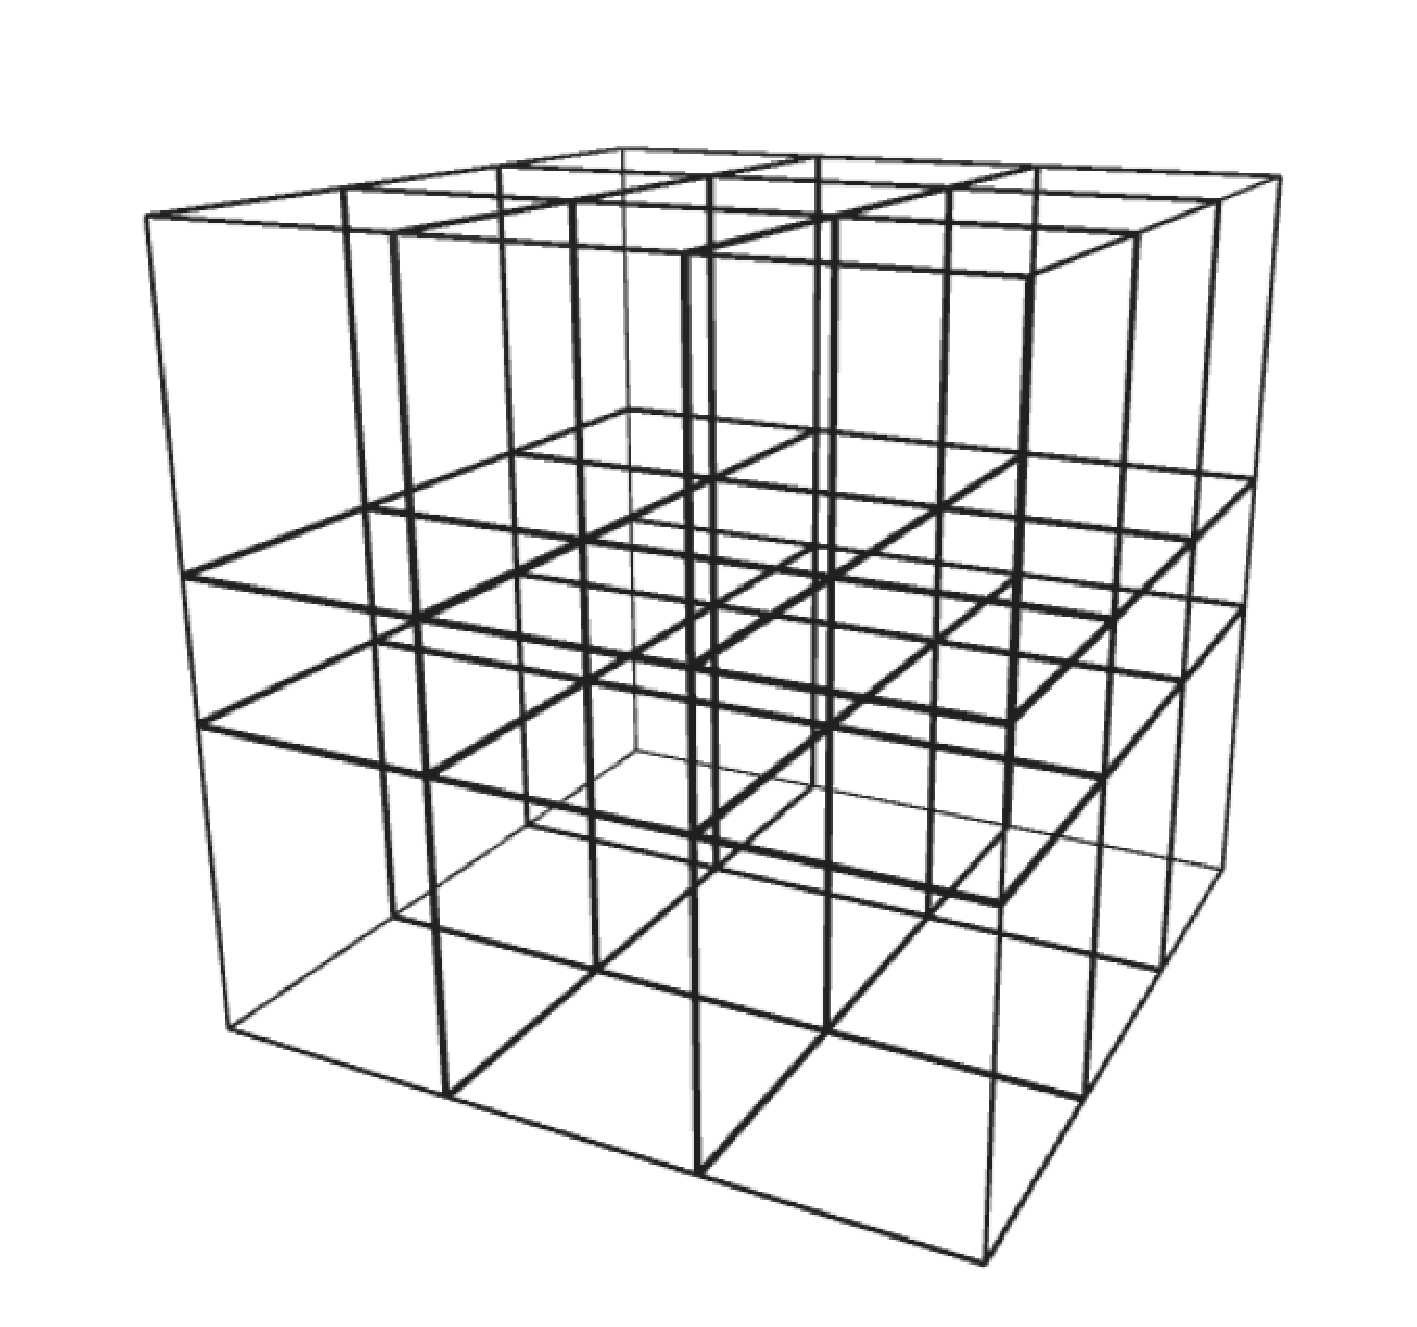
\includegraphics[width=7cm]{figures/mesh.eps}
\end{SCfigure}

\begin{Listing}[h]
	\lstinputlisting[language=fortran]{listings/damaris_example.f90}
	\caption[Example of Fortran simulation using Damaris]{Example of Fortran simulation using Damaris.}
	\label{lst:damarisexample}
\end{Listing}

\begin{Listing}[h]
	\lstinputlisting[language=XML]{listings/damaris_example.xml}
	\caption[Configuration file associated with the Fortran example]{Configuration file associated with the Fortran example.}
	\label{lst:damarisexamplexml}
\end{Listing}

Listing~\ref{lst:damarisexample} is an example of a Fortran program 
that makes use of Damaris. It writes three 1D arrays representing the coordinates of a rectilinear mesh.
At every iteration it then writes
a 3D array representing temperature values on the points of the mesh and sends an event to the dedicated core.
The associated configuration file, shown in Listing~\ref{lst:damarisexamplexml},
describes the data that is expected to be received by the servers, and the
action to perform upon reception of the event. More specifically, lines~14, 15, 16 and 18 of this XML file 
define \emph{layouts}, which describe the type and dimensions of a piece of data. Lines~26 to 33 define a group,
and within this group a set of variables that use these layouts. The temperature variable is defined in line 35.
Finally line~38 associates an event with a function (or \emph{action}) to be
called when the event is received. It also locates the function within a dynamically-loaded library.

The configuration file also contains information for visualization software.
Lines~20 to 24 in the XML file correspond to mesh structure drawn in 
Figure~\ref{fig:mesh}, and built from the three coordinate variables. 
The temperature variable is mapped onto this mesh using its \emph{mesh} attribute.


\section{Evaluation}
\label{sec:evaluation}
We evaluated Damaris with the CM1 atmospheric simulation~\cite{bryan2002benchmark} and ANL's Nek5000 CFD solver~\cite{nek5000}, 
on several platforms: NICS's Kraken~\cite{kraken}, three clusters of the French Grid'5000 platform~\cite{grid5000}, NCSA's BluePrint cluster
and the Blue Waters supercomputer~\cite{bluewaters}. In the following, we first 
evaluate Damaris in the context of improving I/O performance by hiding the I/O variability.
We then evaluate the use of Damaris for several other data management tasks, including data compression, 
I/O scheduling and in situ visualization.

\subsection{Addressing the I/O Bottleneck with Damaris}\label{sec:expIO}

In this first evaluation part, we show how Damaris is used to improve I/O performance.

\subsubsection{Description of the Applications}

The following applications were used in our experiments.
%\begin{SCfigure}[50]
%    \fbox{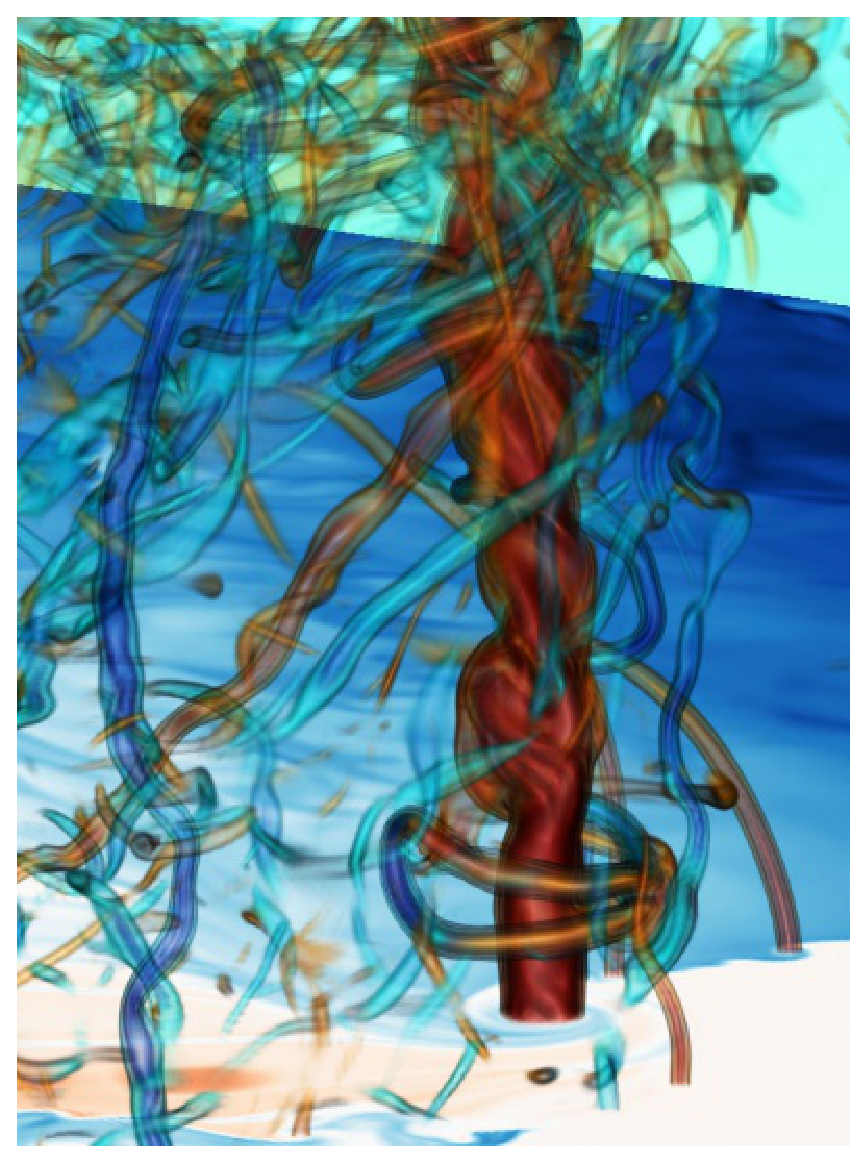
\includegraphics[width=0.38\textwidth,height=0.38\textwidth]{figures/cm1.eps}}
%  \caption[Simulation of a supercell producing a long-track EF5 tornado]{Simulation of a supercell producing a long-track EF5 tornado. 
%  This simulation was realized on NCSA's Blue Waters supercomputer by Leigh Orf (Central Michigan University) 
%  and Bob Wilhelmson (NCSA) using the CM1 code. See~\cite{isgtw-cm1}.}
%\end{SCfigure}

\begin{description}
\item{\textbf{CM1 (Cloud Model 1)}} is used for atmospheric research and is suitable
for modeling small-scale atmospheric phenomena such as thunderstorms
and tornadoes. It follows a typical behavior of scientific simulations,
which alternate computation phases and I/O phases. The simulated domain
is a regular 3D grid representing part of the atmosphere. 
Each point in this domain is characterized by a set of
variables such as local \emph{temperature} or \emph{wind speed}.
CM1 is written in Fortran 90. Parallelization is done using MPI, by
distributing the 3D array along a 2D grid of equally-sized subdomains, each of which
is handled by a process. 
The I/O phase leverages either HDF5 to write one file per
process, or pHDF5~\cite{chilan2006parallel} to write in a shared file in a collective manner.
One of the advantages of using a file-per-process approach is
that compression can be enabled, which cannot be done with pHDF5.
However, at large process counts, the file-per-process approach
generates a large number of files, making all subsequent analysis tasks
intractable.

\item{\textbf{Nek5000}} is a computational fluid dynamics solver based on 
the spectral element method. It is actively developed at ANL's Mathematics 
and Computer Science Division. 
It is written in Fortran 77 and solves its governing equations on an 
unstructured mesh. This mesh consists of multiple 
elements distributed across processes; each element is a small curvilinear mesh.
Each point of the mesh carries
the three components of the fluid's local velocity, as well as other variables.
We chose Nek5000 for this particular meshing structure, different from CM1,
and for the fact that it is substantially more memory-hungry than CM1.
We modified Nek5000 in order to pass the mesh elements and fields data to Damaris.

Nek5000 takes as input the mesh on which to solve the equations, along with 
initial conditions. We call this set a \emph{configuration}. In our
experimental evaluation, we used the \emph{MATiS} configuration, which was
designed to run on 512 to 2048 cores. Another configuration, \emph{turbChannel},
is used in Section~\ref{sec:insitu} to evaluate in situ visualization. This configuration was
designed to run on 32 to 64 cores.
\end{description}

\subsubsection{Platforms and Configurations}

With the CM1 application, our goal was to optimize CM1's I/O for future use on the 
upcoming Blue Waters Petascale supercomputer. Therefore we started with NCSA's IBM Power5 BluePrint 
platform as it was supposed to be representative of Blue Waters' hardware.
On this platform, we evaluated the scalability of the CM1 application with respect to the size of its output, with the file-per-process and 
Damaris approaches. We then experimented on the \emph{parapluie} cluster of Grid'5000's Rennes site.
This cluster features 24-core nodes, which makes it very suitable to our approach based on dedicated cores. 
We then moved our experiments to NICS's Kraken supercomputer, which, in addition to allowing runs at much larger scales, 
has a hardware configuration very close to that of Blue Waters' final design.

With Nek5000, our goal was to confirm the usability of Damaris with a more memory-hungry application.
We completed our experimentation on the \emph{stremi} cluster of Grid'5000's Reims site, which provides the same type
of hardware as the \emph{parapluie} cluster, but a different network.
All these platforms are detailed hereafter, along with the configuration of CM1 and Nek5000 we used.

\begin{description}
\item{\textbf{BluePrint}} is a test platform used at NCSA until 2011 when IBM was still in charge of
delivering the Blue Waters supercomputer.\footnote{As IBM terminated its contract with NCSA in 2011 
and Blue Waters was finally delivered by Cray, BluePrint was later decommissioned and replaced with a 
test platform, JYC, matching the new Blue Waters' design.}
BluePrint features 120 Power5 nodes. Each node consists of 16 cores and 
includes 64~GB of memory. As for its file system, GPFS is deployed on 2 I/O servers.
CM1 was run on 64 nodes (1024 cores), with a $960\times960\times300$-point
domain. Each core handles a $30\times30\times300$-point subdomain with the 
standard approaches, that is, when no dedicated cores are used. 
When dedicating one core out of 16 on each node, computation
cores handle a $24\times40\times300$-point subdomain. On this platform we 
vary the number of variables that CM1 writes, resulting in different sizes of the output.
We enabled the compression feature of HDF5 for all the experiments done on this platform.

\item{\textbf{Grid'5000}} is a French grid testbed. We use its \emph{parapluie} cluster
on the Rennes site and its \emph{stremi} cluster on the Reims site.
On the Rennes site, the parapluie cluster featured 40 nodes of 2~AMD 1.7~GHz CPUs, 12~cores/CPU, 48~GB RAM.
We run CM1 on 28 nodes (672 cores) and 38 nodes (912 cores).
We deployed a PVFS file system on 15 separate I/O servers (2~Intel 2.93~GHz CPUs,
4~cores/CPU, 24~GB RAM, 434~GB local disk). Each PVFS node was
used both as I/O server and metadata server. All nodes (including the file system's) communicate
through a 20G InfiniBand 4x QDR link connected to a common Voltaire switch. 
We use Mpich~\cite{mpich} with ROMIO~\cite{thakur1999data}
compiled against the PVFS library, on a Debian operating system.
The total domain size in CM1 is $1104\times1120\times200$ points, so each core 
handles a $46\times40\times200$-point subdomain with a standard approach, 
and a $48\times40\times200$-point subdomain when one core out of 24 is used by Damaris.

On the Reims site the \emph{stremi} cluster features the same type of node as the \emph{parapluie} cluster.
We run Nek5000 on 30 nodes (720 cores). We deploy PVFS on 4 nodes of the same cluster. Each
PVFS node is used both as I/O server and metadata server. All nodes communicate through a
1G Ethernet network.
We use the MATiS configuration of Nek5000, which contains 695454 elements (small $4 \times 2 \times 4$ curvilinear sub-meshes).
These elements are distributed across available simulation processes. Thus the total number
of elements (and thus the total amount of data output) does not vary whether we use dedicated cores or not.
When no dedicated cores are used, each core handles 965 or 966 such elements. When dedicating one
core out of 24, each simulation core handles 1007 or 1008 elements.

\item{\textbf{Kraken}} is a supercomputer deployed at NICS. It was ranked $11^{th}$ in the 
Top500~\cite{top500} at the time of the experiments, with a peak Linpack performance of 919.1~Teraflops.
It features 9408 Cray XT5 compute nodes connected through a Cray 
SeaStar2+ interconnect and running Cray Linux Environment (CLE). 
Each node has 12 cores and 16~GB of local memory.
Kraken provides a Lustre file system using 336 block storage devices managed
by 48 I/O servers and one metadata server.

On this platform, we studied the weak scalability of the file-per-process,
collective I/O and Damaris approaches in CM1,
that is, we measured how the run time varies with a fixed amount of data per node.
When all cores in each node are used by the simulation, each client process handles a 
$44\times44\times200$-point subdomain.
Using Damaris, each client process (11 per node) 
handles a $48\times44\times200$-point subdomain, which makes the total problem 
size equivalent for a given total number of cores.

\end{description}

\subsubsection{How Damaris Affects the I/O Variability}

\paragraph{Impact of the Number of Cores on the I/O Variability}
We studied the impact of the number of cores on the simulation's write time
with the three I/O approaches: file-per-process, collective I/O, and
Damaris. To do so, we ran CM1 on Kraken with 576, 2304 and 9216 cores.

\begin{SCfigure}[50]
	%\begin{center}
	\includegraphics[width=5.5cm]{figures/kraken-write-time.eps}
	\caption[Write time of CM1 on Kraken]{Duration of a write phase on Kraken (average and maximum).
	For readability reasons we do not plot the minimum write time.
	Damaris shows to completely remove the I/O variability while file-per-process and 
	collective-I/O have a big impact on the run-time predictability.}
	\label{fig:kraken_write_time}
	%\end{center}
\end{SCfigure}

Figure~\ref{fig:kraken_write_time} shows the average and maximum duration of 
an I/O phase on Kraken from the point of view of the simulation.
It corresponds to the time between the two barriers delimiting the I/O phase.
This time is extremely high and variable with Collective I/O, achieving more than 800~seconds
on 9216 cores. The average of 481~seconds still represents about 70\% 
of the overall simulation's run time.

By setting the stripe size to 32~MB instead of 1~MB in Lustre, the write time 
went up to 1600~seconds with a collective I/O approach. This shows that bad choices of 
file system's configuration can lead to extremely poor I/O performance.
Yet it is hard to know in advance the configuration of the file system and
I/O libraries that will lead to a good performance.

Unexpectedly, the file-per-process approach appears to lead to a lower 
variability, especially at large process count, and better performance
than collective I/O.
Yet it still represents an unpredictability (difference between the fastest and 
the slowest phase) of about $\pm 17$ seconds.
For a one month run, writing every 2~minutes would lead 
to an uncertainty of several hours to several days of run time.

When using Damaris, we dedicate one core out of 12 on each 
node, thus potentially reducing the computation performance for the
benefit of I/O efficiency (the impact on overall application performance is 
discussed in the next section). 
As a means to reduce the I/O variability, this approach is clearly effective: 
the time to write from the point of view of the simulation is cut down to the 
time required to perform a series of copies in shared memory. It leads to an apparent write 
time of 0.2~seconds (as opposed to the 481~seconds of collective I/O!) and does not depend anymore on
the number of processes. The variability is in order of $\pm 0.1$ seconds (too small to 
be seen on the figure).

\paragraph{Impact of the Amount of Data on the I/O Variability}
On BluePrint, we vary the amount of data. We aim to compare the file-per-process approach with Damaris
with respect to different output sizes.
%
\begin{SCfigure}[50]
%	\begin{center}
	\includegraphics[width=5.5cm]{figures/blueprint-write-time.eps}
	\caption[Write time of CM1 on BluePrint]{Duration of a write phase (average, maximum and minimum) 
	using file-per-process and Damaris on BluePrint (1024 cores). 
	The amount of data is given in total per write phase.}
	\label{fig:blueprint_write_time}
%	\end{center}
\end{SCfigure}
%
The results are reported in Figure~\ref{fig:blueprint_write_time}.
As we increase the amount of data, the variability
of the I/O time increases with the file-per-process approach. With Damaris however, the 
write time remains in the order of 0.2~seconds for the largest amount of data and 
the variability in the order of $\pm 0.1$ seconds again.

Note that on this platform, data compression was enabled. Thus the observed variability
comes not only from the bottleneck at the file system level, but also from the
different amounts of data that are written across processes and across iterations.
This illustrates the fact that I/O variability does not only comes from the variability of
performance of data transfers and storage, but also on any pre-processing task occurring 
before the actual I/O. Damaris is therefore able to hide this pre-processing variability as well.

\paragraph{Impact of the Hardware}
We studied the impact of the hardware on the I/O variability using Grid'5000's \emph{parapluie}
and \emph{stremi} clusters.
With the large number of cores per node (24) in these clusters as well as a network that is 
substantially less performant than that of Kraken and BluePrint, we aim to illustrate the 
large variation of write time across cores for a single write phase.

We ran CM1 using 672 cores on the \emph{parapluie} cluster, writing a total of 15.8~GB uncompressed data 
(about 24~MB per process) every 20 iterations.
With the file-per-process approach, CM1 reported spending 4.22\% of its time in 
I/O phases. Yet the fastest processes usually terminate their I/O in less than 
1~second, while the slowest take more than 25~seconds.
Figure~\ref{fig:g5k_write_time}~(a) shows the CDF (cumulative distribution function) of write times for one of these write
phases, with a file-per-process approach and with Damaris. 

Finally we ran Nek5000 using 720 cores on the \emph{stremi}, writing a total of 3.5~GB per iteration
using a file-per-process approach.
Figure~\ref{fig:g5k_write_time}~(b) shows the cumulative distribution function of write time 
for one of these write phases with the file-per-process approach and with Damaris. 

In both simulations, we observe a large difference in write time between the fastest
and the slowest process with a file-per-process approach, due to access contention either 
at the level of the network or within the file system. With Damaris however, 
all processes complete their write at the same time. This is due to the absence of contention 
when writing in shared memory.

\begin{figure}
	\begin{center}
	\subfigure[CM1 on Grid'5000 Rennes cluster]{
		\includegraphics[width=5.5cm]{figures/g5k-write-time.eps}
	}\quad
	\subfigure[Nek5000 on Grid'5000 Reims cluster]{
		\includegraphics[width=5.5cm]{figures/nek5-cdf-g5k.eps}
	}
	\caption{Cumulative distribution function of the write time across processes when running CM1 on 672 cores of Grid'5000's Rennes
	cluster and Nek5000 on 720 cores of the Reims cluster.}\label{fig:g5k_write_time}
	\end{center}
\end{figure}

\paragraph{Conclusion} Our experiments show that by replacing write phases with simple copies in 
shared memory and by leaving the task of performing actual I/O to dedicated 
cores, Damaris is able to completely hide the I/O variability from the point of view 
of the simulation, making the application run time more predictable.

%%%%%%%%%%%%%%%%%%%%%%%%%%%%%%%%%%%

\subsubsection{Application's Scalability and I/O Overlap}\label{sec:damaris:scalability}

\paragraph{Impact of Damaris on the Scalability of CM1} CM1 exhibits a very good weak 
scalability and very stable performance when it does not perform any I/O. 
Thus, as we increase the number of cores, the scalability becomes mainly driven by the 
scalability of the I/O phases. To measure the scalability of an approach, 
we define the scalability factor as follows:
\begin{equation}
S = N\times\frac{C}{T_{N}},
\end{equation}
where $N$ is the number of cores considered. We take as a baseline the time 
$C$ of 50 iterations of CM1 on 576 processes without dedicated cores and 
without any I/O. $T_{N}$ is the time CM1 takes to perform 50 iterations
plus one I/O phase, on $N$ cores.
A perfect scalability factor on $N$ cores should be equal to $N$.

The scalability factor on Kraken for the three approaches is given in 
Figure~\ref{fig:scalability}~(a).
Figure~\ref{fig:scalability}~(b) shows the associated application run time 
for 50 iterations plus one write phase.
Damaris enables a nearly perfect scalability where other approaches fail to scale.
In particular, going from Collective I/O to Damaris leads to a $3.5\times$ speedup
on 9216 cores.

\begin{figure}
	\begin{center}
	\subfigure[Scalability Factor on Kraken]{
		\includegraphics[width=5.5cm]{figures/kraken-scalability.eps}
	}\quad
	\subfigure[Run Time on Kraken]{
		\includegraphics[width=5.5cm]{figures/kraken-runtime.eps}
	}
	\caption[Scalability and total run time of CM1 on Kraken]{Scalability factor (a) 
	and overall run time (b) of the CM1 simulation for 50 iterations and 1 write phase, on Kraken.}\label{fig:scalability}
	\end{center}
\end{figure}

\paragraph{Spare Time in Damaris}
Since the scalability of our approach comes from the fact that I/O overlaps with 
computation, we still need to show that the dedicated cores have enough time
to perform the actual I/O while computation goes on.

Figure~\ref{fig:damaris-sparetime} shows the time used by the dedicated cores
to perform the I/O on Kraken and BluePrint with CM1, as well as the time they remain idle,
waiting for the next iteration to complete.

As the amount of data on each node is the same, the only explanation for the 
dedicated cores to take more time at larger process counts on Kraken is the 
access contention for the file system.
On BluePrint the number of processes is constant for each experiment, 
thus the differences in write time come from the different amounts of data.
In all configurations, our experiments show that Damaris spares
a lot of time, during which dedicated cores remain idle. Similar results were obtained on Grid'5000.

\begin{figure}
	\begin{center}
	\subfigure[Write / Idle Time on Kraken]{
	\includegraphics[width=5.5cm]{figures/kraken-damaris-sparetime.eps}
	}
	\quad
	\subfigure[Write / Idle Time on BluePrint]{
	\includegraphics[width=5.5cm]{figures/blueprint-damaris-sparetime.eps}
	}
	\caption[Write and idle time of dedicated cores on Kraken and BluePrint]{Time spent by the 
	dedicated cores writing data for each iteration, and time spared (idle). 
	The spare time is the time dedicated cores are not performing any task.}\label{fig:damaris-sparetime}
	\end{center}
\end{figure}

\begin{SCfigure}[50]
	\includegraphics[width=5.5cm]{figures/nek5-cdf-dc1.eps}
	\caption{CDF of the time spent by dedicated cores writing (statistics across 11 iterations for 30 dedicated cores),
	with Nek5000 on the Reims cluster of Grid'5000.}
	\label{fig:nek5-cdf-dc1}
\end{SCfigure}

With Nek5000, Figure~\ref{fig:nek5-cdf-dc1} shows the CDF of the time spent by dedicated cores writing. 
This time averages to 9.41 seconds, which represents 10\% of overall run time. Thus,
dedicated cores remain idle 90\% of the time. Additionally, this figure shows that the time
spent by dedicated cores writing is stable across iterations and across processes, with a standard deviation of 1.08 seconds.
This stability allows to add additional data processing tasks without worrying about the possibility that
dedicated cores spend an unpredictable time writing.

\paragraph{Conclusion} On all platforms, Damaris shows that it can fully overlap writes 
with computation and still remain idle 75\% to 99\% of time with CM1 (see Figure~\ref{fig:damaris-sparetime}),
and 90\% with Nek5000 (see Figure~\ref{fig:nek5-cdf-dc1}).
Thus, without impacting the application, it becomes possible to further increase the 
frequency of output, or to perform additional data processing operations such as in situ data analysis and visualization. 

\subsubsection{Effective I/O Throughput}\label{sec:throughput}

We then studied the effect of Damaris on the aggregate throughput observed from the computation nodes to
the file system. Note that in the case of Damaris, this throughput is only observed by the 
dedicated cores.

\begin{SCfigure}[50]
	\includegraphics[width=5.5cm]{figures/kraken-throughput.eps}
	\caption[Aggregate throughput of CM1 on Kraken]{Average aggregate 
	throughput achieved on Kraken with the different 
	approaches. Damaris shows a 6 times improvement over the file-per-process 
	approach and 15 times over Collective I/O on 9216 cores.}
	\label{fig:throughput-kraken}
\end{SCfigure}

Figure~\ref{fig:throughput-kraken} presents the aggregate throughput obtained by CM1
with the three approaches on Kraken.
At the largest scale (9216 cores) Damaris achieves an aggregate throughput about 6 times
higher than the file-per-process approach, and 15 times higher than collective I/O.
The results obtained on 672 cores of Grid'5000 are presented in 
Table~\ref{tab:grid5000_throughput}.
The throughput achieved with Damaris here is more than 6 times higher than the other two approaches.
Since compression was enabled on BluePrint, we do not provide the resulting 
throughputs, as it depends on the overhead of the compression algorithm used
and the resulting size of the data.

\begin{SCtable}[50]
%\center
\begin{tabular}{|r|c|}
  \hline
   & Aggregate throughput \\
   \hline
    File-per-process & 695~MB/s \\
    Collective-I/O & 636~MB/s \\
    Damaris & 4.32~GB/s \\
  \hline
\end{tabular}
\caption[Average aggregate throughput of CM1 on Grid'5000]{Average 
aggregate throughput on Grid'5000's \emph{parapluie} cluster, with CM1 running on 672 cores.}\label{tab:grid5000_throughput}
\end{SCtable}

With Nek5000 on the \emph{stremi} cluster of Grid'5000, 
Table~\ref{tab:nek5_throughput} shows that Damaris enables a $4.6 \times$ increase
of throughput, going from 73.5~MB/s with the file-per-process approach, to 337.6~MB/s with one dedicated
core per node. 

\begin{SCtable}[50]
%\center
\begin{tabular}{|r|c|}
  \hline
   & Aggregate throughput \\
   \hline
    File-per-process & 73.5~MB/s \\
    Damaris & 337.6~MB/s \\
  \hline
\end{tabular}
\caption{Average aggregate throughput on Grid'5000's \emph{stremi} cluster, with Nek5000 running on 720 cores.}\label{tab:nek5_throughput}
\end{SCtable}

\paragraph{Conclusion} By avoiding process synchronization and 
access contention at the level of a node and by gathering data into bigger 
files, Damaris reduces the pressure on metadata servers and issues bigger operations
that can be more efficiently handled by storage servers. As a result, on 
all platforms and with each simulation, Damaris substantially increases the aggregate 
throughput, thus making a more efficient use of the file system.

\subsubsection{Improvements: Leveraging the Spare Time}

Section~\ref{sec:damaris:scalability} showed that, with both applications, 
dedicated cores remain idle most of the time.
In order to leverage the spare time in dedicated cores, we implemented two improvements:
compression, and transfer delays. These improvements are evaluated hereafter in the
context of CM1. Again here, Damaris aggregates data to write one file per dedicated core. 

\paragraph{Compression} 
We used dedicated cores to compress the output data prior to writing it.
Using lossless gzip compression, we observed a compression ratio of 187\%. 
When writing data for offline visualization, atmospheric scientists can afford to reduce the floating point precision
to 16~bits, as it does not visually impact the resulting images. 
Doing so leads to nearly 600\% compression ratio when coupling with gzip. 
On Kraken, the time required by dedicated cores to compress and write data was
twice longer than the time required to simply write uncompressed data. Yet 
contrary to enabling compression in the file-per-process 
approach, the overhead and jitter induced by the compression phase is 
completely hidden within the dedicated cores, and do not impact the running 
simulation. In other words, \emph{compression is offered for free} by Damaris.

\paragraph{Data Transfer Delays}
Additionally, we implemented in Damaris the capability to
delay data movements. The algorithm is very simple and does not involve any
communication between processes: each dedicated core computes
an estimation of the duration of an iteration of the simulation by measuring the time between
two consecutive calls to \texttt{damaris\_end\_iteration} (about 230~seconds on Kraken). 
This time is then divided into as many slots as there are dedicated cores. Each dedicated 
core waits for its slot before writing. This avoids access contention at the level 
of the file system. We evaluated this strategy on 2304 cores on Kraken, the aggregate 
throughput reaches 13.1~GB/s on average, instead of 9.7~GB/s when this 
algorithm is not used.

\paragraph{Summary}
These two improvements have also been evaluated on 912 cores of Grid'5000.
All results are synthesized in Figure~\ref{fig:damaris-improvement},
which shows the average write time in dedicated cores.
The delay strategy reduces the write time in both platforms.
Compression however introduces an overhead on Kraken, thus we are 
facing a tradeoff between reducing the 
storage space used or reducing the spare time.
A potential optimization would be to enable or disable compression
at run time depending on the need to reduce write time or storage space.

\begin{SCfigure}[50]
%	\begin{center}
	\includegraphics[width=5.5cm]{figures/gzip-scheduling-improvements.eps}
	\caption[Write time in Damaris using compression and transfer delays]{Write 
	time in the dedicated cores when enabling compression or transfer delays.} 
	\label{fig:damaris-improvement}
%	\end{center}
\end{SCfigure}


\subsection{Using Damaris for In Situ Visualization}\label{sec:insitu}

Far from being restricted to performing I/O, Damaris can also leverage
the high-level description of data provided in its configuration file
to feed in situ visualization pipelines. In the following we evaluate
such use of Damaris for in situ visualization. We highlight two aspects: scalability
of the visualization algorithms when using dedicated cores, and impact
of in situ visualization on application run time.

\subsubsection{Platforms and Configurations}

We use again the CM1 and Nek5000 applications
presented in the previous sections, respectively on Blue Waters and Grid'5000.
The platforms and configurations of the experiments are described hereafter.

\begin{description}
\item{\textbf{Blue Waters}}
Blue Waters~\cite{bluewaters} is a 13.3-petaflops supercomputer deployed at NCSA.
It features 26,864 nodes in 237 Cray XE6 cabinets
and 44 Cray XK7 cabinets, running Cray Linux Environment (CLE). 
We leveraged the XE6 nodes, each of which features 16 cores.
\end{description}

\paragraph{Methodology with CM1 on Blue Waters}
CM1 requires a long run time before an interesting atmospheric phenomenon appears,
and such a phenomenon may not appear at small scale. Yet contrary to the evaluation of
I/O performance, we need visualizable phenomena to appear in order to evaluate the 
performance of in situ visualization tasks.
Thus we first ran CM1 with the help of atmospheric
scientists to produce relevant data. We generated a representative dataset of 
$3840 \times 3840 \times 400$ points spanning several iterations.

We then extracted the I/O kernel 
from the CM1 code and built a program that replays its behavior at a given scale 
and with a given resolution by reloading, redistributing and interpolating the 
precomputed data.
The I/O kernel, identical to the I/O part of the simulation, calls Damaris
functions to transfer the data to Damaris. Damaris then performs in situ visualization
through a connection to VisIt's \emph{libsim} library~\cite{whitlock2011parallel}, 
either in a time-partitioning manner or using dedicated cores.
Our goal with CM1 is to show the interplay between the scalability of the
visualization tasks and the use of dedicated cores to run them.

\paragraph{Methodology with Nek5000 on Grid'5000}
With Nek5000, we used the \emph{stremi} cluster of Grid'5000 already presented
in the previous section. In addition to the \emph{MATiS} configuration, we also
use the \emph{turbChannel} configuration, which runs at smaller scales and is
more appropriate for interactive in situ visualization.
Our goal with Nek5000 is to show the impact of in situ visualization on the variability of
the application's run time.

\paragraph{Using Damaris in Time-Partitioning Mode} In order to
compare the traditional ``time-partitioning'' approach with the use of dedicated
cores enabled by Damaris, we added a time-partitioning mode in Damaris. This mode,
which can be enabled through the configuration file, prevents Damaris from
dedicating cores, and runs all plugins in a synchronous manner on all cores
running the simulation. This mode allows us to compare the traditional time-partitioning
in situ visualization approach with the use of dedicated cores without having to modify the simulations
twice.

\begin{figure}[t]
\centering
	\subfigure[CM1 Isosurface]{
	\fbox{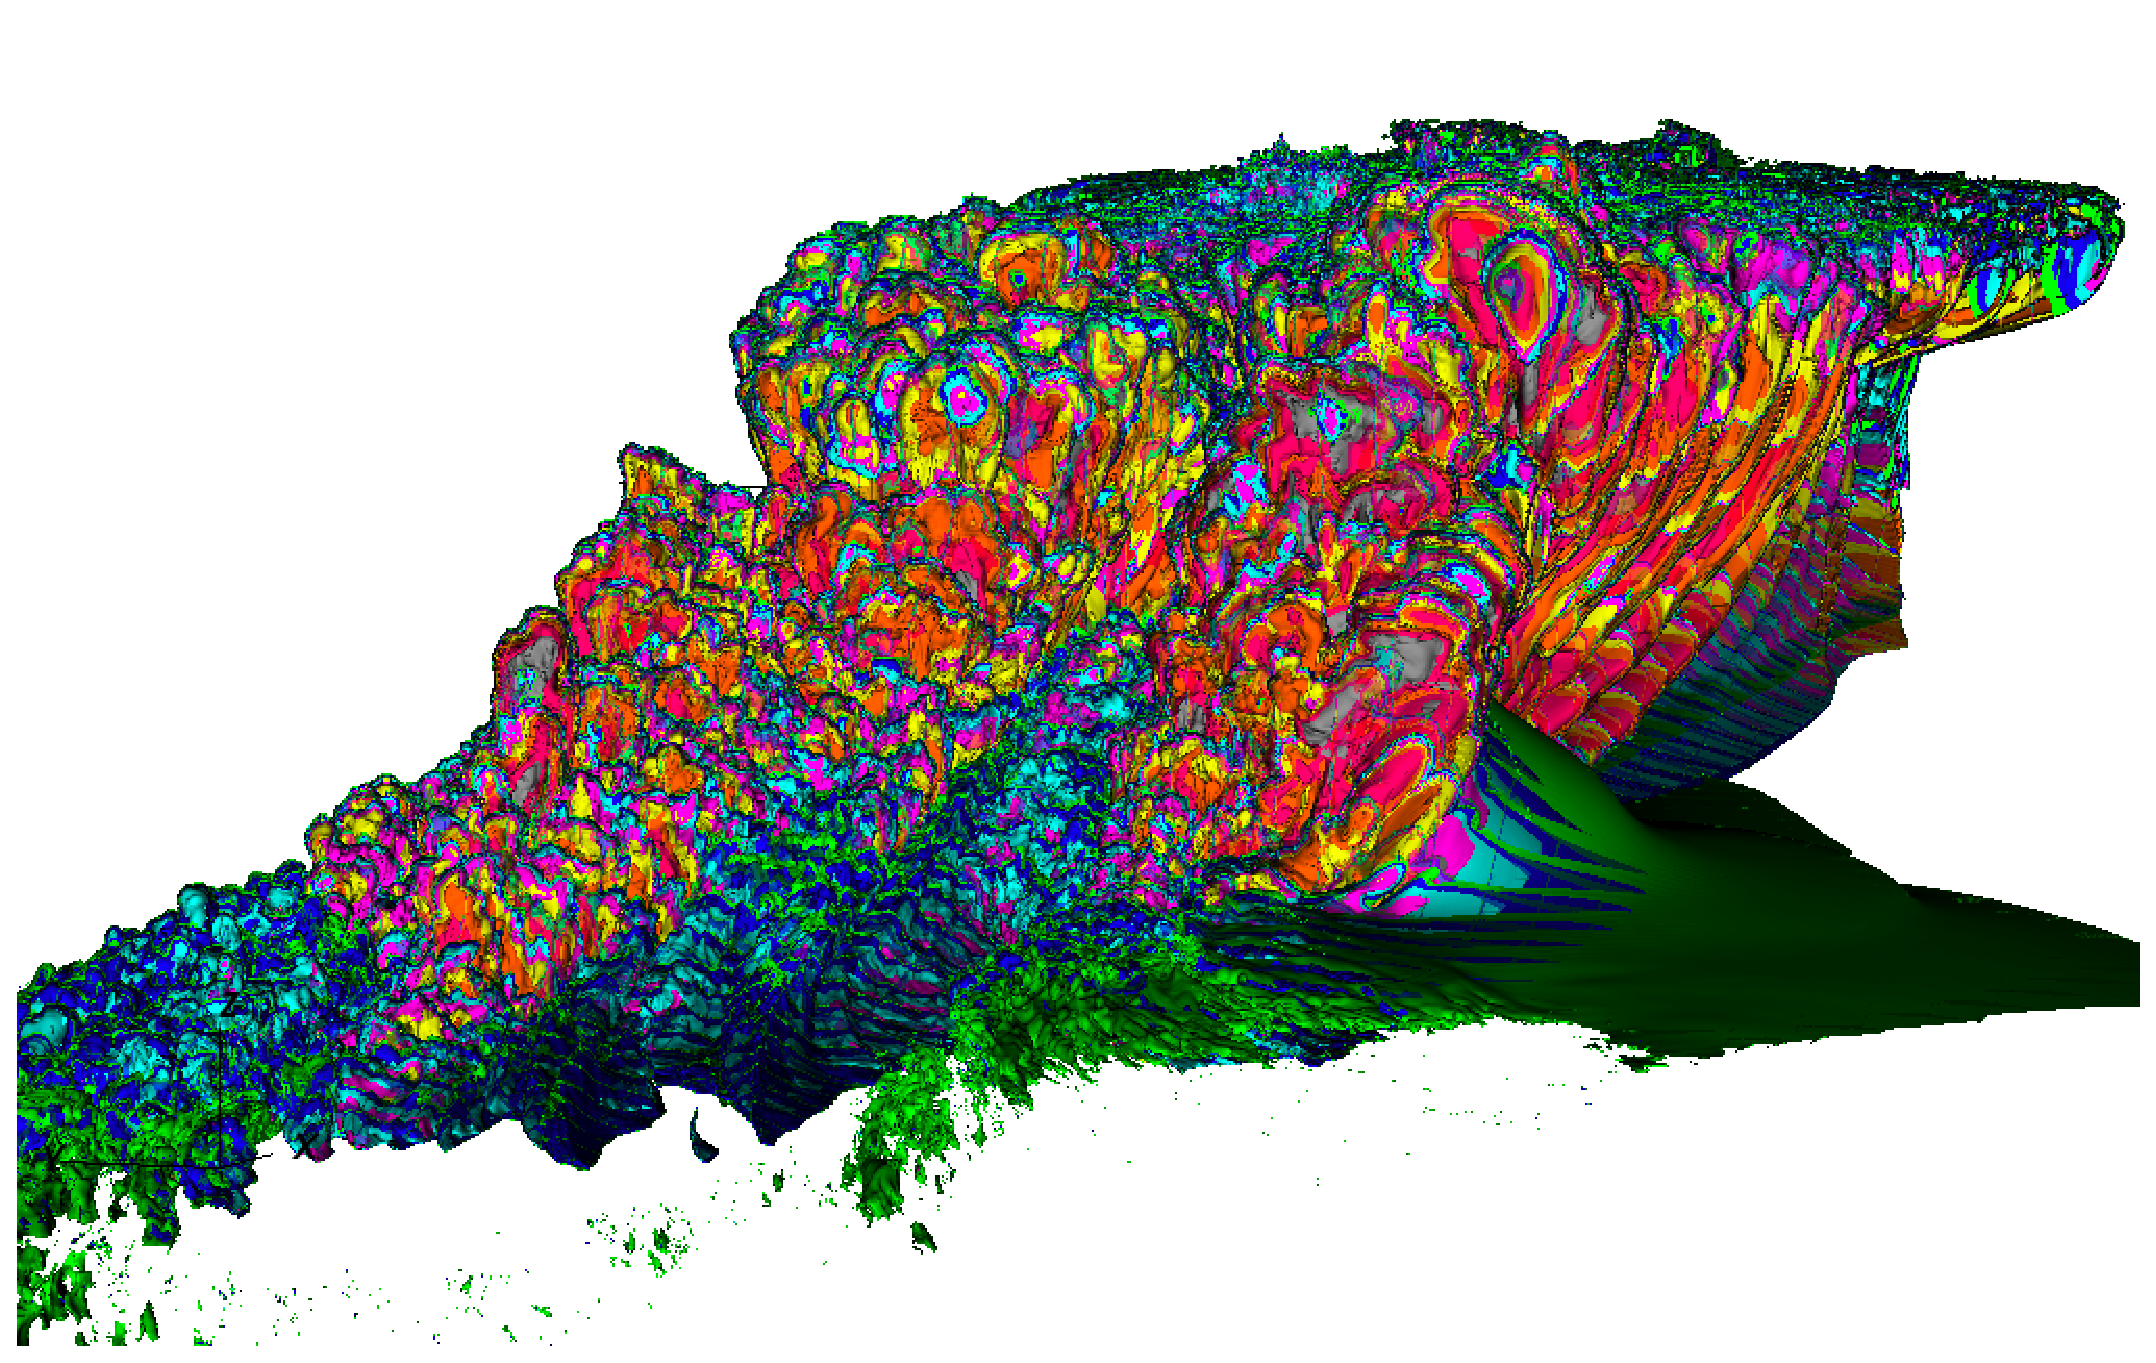
\includegraphics[width=3.5cm,height=3.5cm]{figures/cm1-isosurface.eps}}}
	\subfigure[CM1 Ray Casting]{
	\fbox{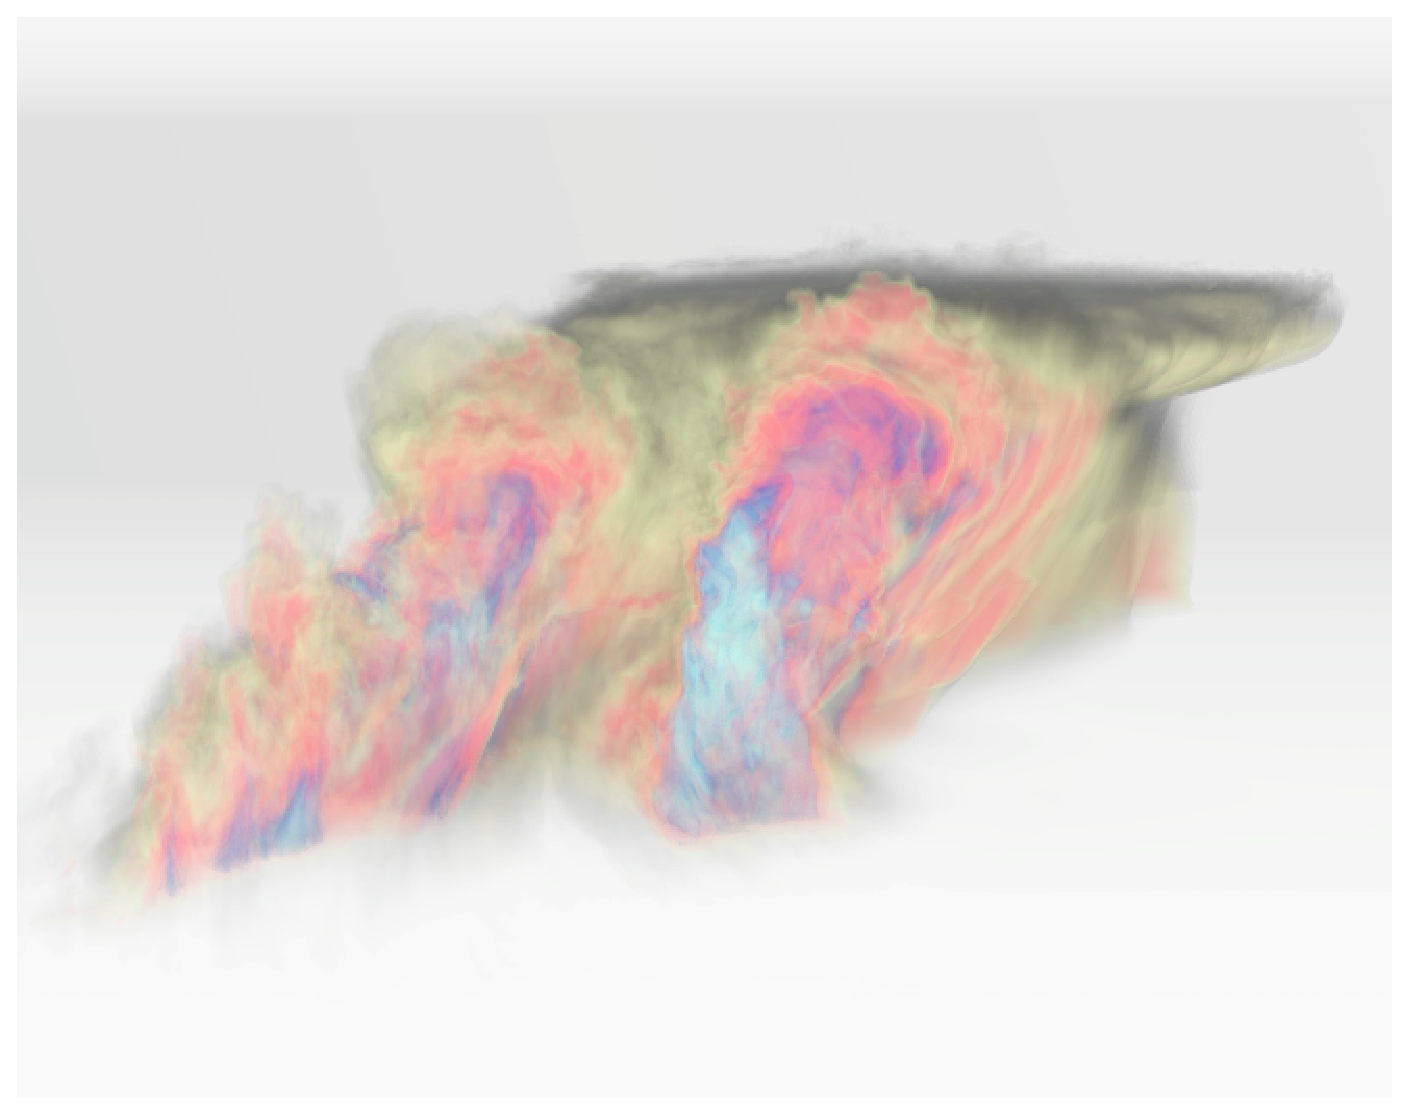
\includegraphics[width=3.5cm,height=3.5cm]{figures/cm1-raycasting.eps}}}
	\subfigure[Nek5000 Isosurface]{
	\fbox{\includegraphics[width=3.5cm,height=3.5cm]{figures/nek5-volume.eps}}}
	
	\caption{Example results obtained in situ with Damaris:
	(a) 10-level isosurface of the DBZ variable on 6400 cores (Blue Waters).
	(b) Ray-casting of the \emph{dbz} variable on 6400 cores (Blue Waters).
	(c) Ten-level isosurface of the $y$ velocity field in 
	the TurbChannel configuration of Nek5000.}\label{fig:visualresults}
\end{figure}

\subsubsection{Impact of Dedicated Cores on the Scalability of Visualization Tasks}

With CM1 on Blue Waters, we measured the time (average of 15 
iterations) to complete either an isosurface rendering or a ray casting
rendering using time partitioning and dedicated cores for each scenario. 
The comparative results are reported in Figure~\ref{fig:cm1vistime}.

\begin{figure}[t]
\centering
	\subfigure[In Situ Isosurface]{
	\includegraphics[width=5.5cm]{figures/cm1-in-situ-isosurface.eps}}
	\quad
	\subfigure[In Situ Ray Casting]{
	\includegraphics[width=5.5cm]{figures/cm1-in-situ-ray-casting.eps}}
	\caption{Rendering time using ray-casting and isosurfaces, with 
	time-partitioning and dedicated cores with CM1. Note that the number of cores 
	represents the total number used for the experiments; using a dedicated-core 
	approach, 1/16 of this total number is effectively used for in situ visualization,
	which explains the overall higher rendering time with dedicated cores.}
	\label{fig:cm1vistime}
\end{figure}

The isosurface algorithm (resulting image presented in Figure~\ref{fig:visualresults} (a))
scales well with the number of cores 
using both approaches. A time-partitioning approach would thus be 
appropriate if the user does not need to hide the run time impact of in situ 
visualization.
However, on 6400 cores, it takes as much time 
to complete the rendering as on 400 dedicated cores. In
terms of pure computational efficiency, an approach based on dedicated cores is thus 16 
times more efficient.

The ray-casting algorithm (resulting image presented in Figure~\ref{fig:visualresults} (b))
on the other hand has a poorer scalability. After 
decreasing, the rendering time goes up again at a 6400-core scale, and it 
becomes about twice more efficient to use a reduced number of dedicated 
cores to complete this same rendering.

\paragraph{Conclusion} The choice of using dedicated cores versus a time-partitioning in situ visualization approach 
depends on (1) the intended visualization scenario, (2) the scale of the experiments and 
(3) the intended frequency of visual output. Our experiments show that at small scale,
the performance of rendering algorithms are good enough to be executed in a time-partitioning manner,
provided that the user is ready to increase the run time of his simulation. At large scale however,
it becomes more efficient to use dedicated cores, especially when using ray-casting,
where the observed rendering performance is substantially better when using a reduced number of
processes.

\subsubsection{Impact of In Situ Visualization on Run Time Variability}

Our goal in this series of experiments is to show the impact of in situ visualization
tasks on the run-time variability of the simulation, and to show how dedicated cores
help alleviate this variability. We show in particular the effect of 
interactivity on this variability. We use Nek5000 for this purpose.
 
Figure~\ref{fig:visualresults}~(c) shows the result of a 10-level 
isosurface rendering of the fluid velocity along the $y$ axis, with the 
TurbChannel case. We use the MATiS configuration to show the scalability of our 
approach based on Damaris against a standard, time-partitioning approach.

\paragraph{Results with the TurbChannel Configuration}
To assess the impact of in situ visualization on the run time, we run 
TurbChannel on 48 cores using the two approaches: first we use a 
time-partitioning mode, in which all 48 cores are used by the simulation and 
synchronously perform in situ visualization. Then we switch on one dedicated core per node,
leading to 46 cores being used by the simulation while 2 cores asynchronously run 
the in situ visualization tasks.

In each case, we consider four scenarios: 
\begin{enumerate}
	\item The simulation runs without visualization;
	\item A user connects VisIt to the simulation but does not ask for any output;
	\item The user asks for isosurfaces of the velocity fields but does not interact with VisIt any further 
	(letting the Damaris/Viz update the output after each iteration);
	\item The user has heavy interactions with the simulations (for example rendering different variables, 
using different algorithms, zooming on particular domains, changing the 
resolution).
\end{enumerate}

Figure~\ref{fig:nek5variability} presents a trace of the duration of each
iteration during the four aforementioned scenarios using the two approaches.
Figure~\ref{fig:nek5variability}~(a) shows that in situ visualization using 
a time-partitioning approach has a large impact on the 
simulation run time, even when no interaction is performed. The simple act of connecting
VisIt without rendering anything forces the simulation to at least update metadata at each iteration,
which takes time.
Figure~\ref{fig:nek5variability}~(b) shows that in situ visualization based on dedicated cores, 
on the other hand, is completely transparent from the point of view of the simulation.

\begin{figure}[t]
\centering
	\subfigure[Time-Partitioning]{
	\includegraphics[width=5.5cm]{figures/turbchannel-time-partitioning.eps}}
	\quad
	\subfigure[Dedicated Cores]{
	\includegraphics[width=5.5cm]{figures/turbchannel-space-partitioning.eps}}
	\caption[Run-time variability in CM1 due to in situ visualization]{Variability 
	in run time induced by different scenarios of in situ 
	interactive visualization.}\label{fig:nek5variability}
\end{figure}

\paragraph{Results with the MATiS Configuration}
We ran the MATiS configuration on 816 cores of the \emph{stremi} cluster. Each 
iteration takes approximately one minute and due to the size of the
mesh, it is difficult to perform interactive visualization. 
Therefore we connect VisIt and simply query for a 3D pseudo-color plot of the $vx$ 
variable ($x$ component of the fluid velocity) that is then continuously updated.
For the following results, the time-partitioning approach outputs one image every time step,
while dedicated cores adapted the output frequency to one image every 25 
time steps in order to avoid blocking the simulation when the shared memory buffer becomes full.

Figure~\ref{fig:matisruntime} reports the behavior of the application with and 
without visualization performed, and with and without dedicated cores. 
Corresponding statistics are presented in Table~\ref{tab:matisstats}.

\begin{figure}[t]
\centering
	\subfigure[Time Partitioning, Without Visualization]{
	\includegraphics[width=5.5cm]{figures/matis-tp-no-viz.eps}}
	\quad
	\subfigure[Time Partitioning, With Visualization]{
	\includegraphics[width=5.5cm]{figures/matis-tp-viz.eps}}
	\subfigure[Space Partitioning, Without Visualization]{
	\includegraphics[width=5.5cm]{figures/matis-sp-no-viz.eps}}
	\quad
	\subfigure[Space Partitioning, With Visualization]{
	\includegraphics[width=5.5cm]{figures/matis-sp-viz.eps}}
	\caption[Iteration time of Nek5000's MATiS configuration with and without in situ visualization]{Iteration time 
	of the MATiS configuration without visualization 
	(left) and with visualization enabled (right).
	Top: with time partitioning, visualization time adds to the simulation time. 
	Bottom: With dedicated cores, visualization time entirely overlaps with simulation time.}\label{fig:matisruntime}
\end{figure}

\begin{table}
	\center
\caption[Average iteration time of Nek5000's MATiS configuration]{Average 
	iteration time of the Nek5000 MATiS configuration with a
   time-partitioning approach and with dedicated cores, with and without 
   visualization.\vspace{0.5cm}}\label{tab:matisstats}
   \begin{tabular}{|l|l|c|c|}
   \hline
\textbf{Iteration Time} & & Average & Std. dev. \\
	\hline
\multirow{2}{*}{Time Partitioning} & w/o vis. & 75.07 sec  & 22,93 \\
	& with vis. & 205.21 sec & 57.15 \\
	\hline
\multirow{2}{*}{Space Partitioning} & w/o vis. & 67.76 sec & 20.09 \\
	& with vis. & 64.79 sec  & 20.44 \\
	\hline
   \end{tabular}
\end{table}

\paragraph{Conclusion} Time-partitioning visualization not only increases the average run time but 
also increases the standard deviation of this run time, making it more unpredictable.
On the other hand, the approach based on dedicated cores yields more consistent results.
One might expect dedicated cores to interfere with the
simulation as it performs intensive communications while the simulation runs. 
However, in practice we observe very little such run time variation.

We also remark that decreasing the number of cores used by the simulation can actually
decreases its run time. For instance with Nek5000 on Grid'5000, the simulation reaches the
limit of its scalability. Yet due to its memory requirements and the amount of memory available
in each node of this platform, it is still necessary to run
it on this number of nodes. In other words, as reducing the number of cores per node
actually used by the simulation increases its performance, it further motivates the
use of these spare cores for extra tasks such as visualization.

Finally, while the time-partitioning approach performs visualization at every 
time step here, dedicated cores have adapted the frequency of 
its output to 1 image every 25 time steps.
If a time-partitioning approach were to only output 1 image every 25 time steps 
(which corresponds to having only the $25^{th}$ iteration being impacted 
in Figure~\ref{fig:matisruntime} (b)), the completion time for 25 time steps 
would be 2007 seconds on average.
With dedicated cores, this takes 1620 seconds, that is, a 20\% speedup. 
Furthermore, since dedicated cores enable the visualization and 
simulation tasks to overlap, the total run time is unchanged with the addition of in situ visualization.

%\subsection{Using Damaris for In Situ Visualization}\label{sec:insitu_eval}

In this section, we evaluate how Damaris can be used for in situ visualization by
studying two aspects of our framework. First we show the adaptability
and ease of use of Damaris by quantifying required code modifications for data accesses
in existing simulations. 
We then evaluate the performance benefits of using 
dedicated cores in terms of scalability of the visualization process,
and impact on simulation performance.

\subsubsection{Impact on Code Instrumentation and Adaptability}

We compared our framework with two representative software packages 
used for tightly-coupled ISV, VisIt and ParaView, 
in terms of code modification and adaptability. 
We conducted this study around the particular 
scenario of a rectilinear mesh with temperature values. This scenario, 
corresponds to the sample code presented in Section~\ref{sec:damaris_viz:DamarisInSitu}.
It will also be applied in  Section~\ref{sec:damaris_viz:Experiments} to the CM1 
simulation, and is characteristic of a climate simulation handling a 3D 
\emph{temperature} array of double precision values mapped onto a rectilinear grid.
%Listing~\ref{lst:basesim} introduces the corresponding portion of the simulation
%code where these arrays are allocated.

%\begin{Listing}[t]
%	\lstinputlisting[language=C]{listings/base_sim.c}
%	\caption{Data allocation in the original simulation.}\label{lst:basesim}
%\end{Listing}

%Section~\ref{sec:DamarisInSitu:visit} presented how this scenario is handled
%by our framework through a six-lines code instrumentation and a short XML 
%description. In the following we compare this instrumentation to two widely used
%software: VisIt and ParaView.

\paragraph{Damaris vs. VisIt}
VisIt is one of the major software for
parallel scientific visualization. It offers in situ visualization capabilities through the 
\emph{libsim}~\cite{whitlock2011parallel} library. This library allows the simulation 
to act as a parallel rendering engine when receiving commands from a VisIt client.
Visualization tasks can also be scripted to run 
without user intervention. VisIt works directly on the data provided by 
the simulation without making a copy. 
%This leads to a major reduction of memory requirements. 
The ``Getting data into VisIt'' manual~\cite{gettingdataintovisit}
provides a complete documentation on how to instrument a simulation. This 
instrumentation requires to restructure the simulation's main loop in order to 
periodically check for pending visualization requests from the user, using the 
\texttt{VisItDetectInput(...)} function. When a connection is started with a 
client, the simulation has to provide callback functions to the \emph{libsim} 
library. These callbacks access data, metadata and issue commands. 
In our example, two callback functions are provided in addition to the callback 
functions required for metadata access and response to commands. 
Listing~\ref{lst:visitaccess} presents an overview of these data access functions.

%%%%%%%%%%%%%%%%%%%%%%%%%%%
\begin{Listing}[t]
	\lstinputlisting[language=C]{listings/visit_access.c}
	\caption[In situ data access functions using VisIt]{Data access functions 
	for our sample application using VisIt. The 
	first function retrieves the mesh coordinates, while the second retrieves 
	the temperature field. The two last lines register the two functions as 
	callbacks handling data accesses. This sample code does not show the 
	modifications to the simulation's main loop.}
	\label{lst:visitaccess}
\end{Listing}

In contrast, the code modifications required by Damaris boil down to the few
lines presented in Listing~\ref{lst:damarisaccess} in Section~\ref{sec:damaris_viz:DamarisInSitu}.

In addition to our previous example and to quantify more precisely the modification costs
in VisIt and in Damaris, we rewrote the examples provided in 
VisIt's source to work with Damaris. Table~\ref{tab:instrumentation:visit}
summarizes the number of lines of code required to instrument these examples 
with the two frameworks.\footnote{These numbers might differ our previous work~\cite{dorier2013damarisviz}, 
as a newer version of Damaris with a slightly different API was used here.} 
We removed all comments and blank lines in order to
count only the lines of code relevant to the simulation/visualization coupling. 
Note that all of these examples except the 
last are serial. The last one, \emph{life.c}, requires further 
modifications with VisIt to provide callback functions for collective communications.
All these codes (including the unmodified ones from VisIt) are available in the 
Damaris release.\footnote{See \url{http://damaris.gforge.inria.fr}.}

\begin{SCtable}
%\center
 \caption[Amount of code modifications in example codes using VisIt and Damaris]{Code 
   modifications of different VisIt examples. Damaris requires
   code modifications and an external XML file.}\label{tab:instrumentation:visit}
   \begin{tabular}{|l|c|c|c|}
      \hline
   & \textbf{VisIt} & \multicolumn{2}{c|}{\textbf{Damaris}} \\
      \hline
Simulation   & C  & C & XML \\
      \hline
      curve.c  & 144 lines & 8  lines & 32 lines\\
      mesh.c   & 167 lines & 10 lines & 46 lines\\
      var.c    & 271 lines & 15 lines & 63 lines\\
	  point.c  & 161 lines & 9  lines & 33 lines\\
	  blocks.c & 188 lines & 10 lines & 45 lines\\
      life.c   & 305 lines & 10 lines & 40 lines\\
      \hline
   \end{tabular}
   
\end{SCtable}

These number of lines clearly show that Damaris greatly simplifies the code
modifications required to couple existing simulations with visualization tools,
thus helping users adopt in situ visualization as an alternative to offline
visualization.

\paragraph{Damaris vs. ParaView}
Like VisIt, ParaView is based on VTK. 
The ParaView in situ interface, called \emph{Catalyst}\footnote{See \url{http://catalyst.paraview.org/}.} 
or \emph{co-processing library}~\cite{fabian2011paraview} integrates a visualization pipeline 
(written in C++ or in Python) into the simulation. The simulation periodically 
feeds this predefined pipeline with data in order to produce visualization 
outputs, for example images.

While VisIt's \emph{libsim} is based on callback functions and works in C, C++ 
and Fortran, Catalyst requires the simulation to wrap 
its data into VTK C++ objects. One solution consists of writing C++ classes that 
inherit from the right VTK objects such as \texttt{vtkDoubleArray}. Another is 
to write functions that wrap the original data by creating instances of existing
VTK classes. This solution is especially more appropriate when it comes to 
instrumenting C or Fortran simulations. Indeed ParaView does not provide any C or 
Fortran binding, leaving the developer with the difficult task of bridging the languages.
Listing~\ref{lst:paraviewaccess} summarizes the main steps in creating the
right VTK objects for our sample application.

\begin{Listing}
	\lstinputlisting[language=C]{listings/paraview_access.cpp}
	\caption[In situ data access functions using ParaView]{Data access functions for our sample application using ParaView. 
	The first function wraps the temperature field into the VTK object which is used by 
	the second function that adds information related to the mesh coordinates. 
	This code does not show all the additional codes required to initialize
	the visualization pipeline.
	}\label{lst:paraviewaccess}
\end{Listing}

The advantage of an \emph{a priori} definition of the visualization pipeline in 
ParaView is the possibility to start a simulation and be able to periodically
check the generated images. The downside is the lack
of interactivity and flexibility at run time of the visualization tasks. 
Note also that part of the ParaView pipeline can be relocated to 
a visualization cluster. This case is out of the scope of our work.

Other visualization software such as ezViz have a C or C++ API that
can be used to perform in situ visualization in a way similar to ParaView and VisIt.

A first attempt to provide in situ visualization through VTK objects was done
with the Nek5000 simulation. The
VTK code was made of 600 lines of C++ code, that we reduced to 20 lines of
Fortran with Damaris, along with 60 lines of XML, for the same visual result 
using VisIt as a backend.

%\subsection{The Case of Enzo and YT}

%Finally, we studied how Damaris would compare to a simulation that already uses
%in situ visualization. We choose the Enzo~\cite{enzo} code for this purpose.

%Enzo is a well known astrophysical simulation based on adaptive mesh
%refinement (AMR). 
%The particular needs of the Enzo community in terms of visualization led to
%the 
%development of the YT~\cite{yt} package, a Python library working on top of 
%Matplotlib and supporting most visualization scenarios of AMR simulations. 
%YT was
%originally designed to work as an offline visualization package, fed with
%Enzo's 
%output files. Yet in recent versions of Enzo, interesting developments have
%been
%made towards in situ visualization capabilities.

%The current version of Enzo\footnote{Version 2.1 as we write this thesis.} 
%periodically wraps its data and metadata hierarchy into Python 
%structures, in particular NumPy arrays. It then calls a user-provided Python 
%script from which these information can be accessed for in situ analysis 
%purpose. Wrapping Enzo structures in Python represents about 800 lines of C++ 
%code spread in five different files, where Damaris would require less than
%100 lines. This number is based on manually counting the number of 
%variables that Enzo exposes to Python, knowing that Damaris would require at
%most two lines of code per variable. Some of these variables are however cosmological or 
%structural constants that can be supplied directly within the configuration file.
%The actual number of lines required should thus be even lower.

%The aforementioned in situ visualization scenario is specific to Enzo and uses 
%its YT package. Yet any simulation developer could use these techniques to offer 
%in situ analysis capabilities to his application. Damaris alleviates the task of 
%building the C/Python interface.


%%%%%%%%%%%%%%%%%%%%%%%%%%%%%%%%%%%%%%%%%%%%%%%%%%%%%%%%%%%%%%%%%%%%%%%%%%%%%%%%
%%%%%%%%%%%%%%%%%%%%%%%%%%%%%%%%%%%%%%%%%%%%%%%%%%%%%%%%%%%%%%%%%%%%%%%%%%%%%%%%
%%%%%%%%%%%%%%%%%%%%%%%%%%%%%%%%%%%%%%%%%%%%%%%%%%%%%%%%%%%%%%%%%%%%%%%%%%%%%%%%
%%%%%%%%%%%%%%%%%%%%%%%%%%%%%%%%%%%%%%%%%%%%%%%%%%%%%%%%%%%%%%%%%%%%%%%%%%%%%%%%
%%%%%%%%%%%%%%%%%%%%%%%%%%%%%%%%%%%%%%%%%%%%%%%%%%%%%%%%%%%%%%%%%%%%%%%%%%%%%%%%
%%%%%%%%%%%%%%%%%%%%%%%%%%%%%%%%%%%%%%%%%%%%%%%%%%%%%%%%%%%%%%%%%%%%%%%%%%%%%%%%
%%%%%%%%%%%%%%%%%%%%%%%%%%%%%%%%%%%%%%%%%%%%%%%%%%%%%%%%%%%%%%%%%%%%%%%%%%%%%%%%
%%%%%%%%%%%%%%%%%%%%%%%%%%%%%%%%%%%%%%%%%%%%%%%%%%%%%%%%%%%%%%%%%%%%%%%%%%%%%%%%
%%%%%%%%%%%%%%%%%%%%%%%%%%%%%%%%%%%%%%%%%%%%%%%%%%%%%%%%%%%%%%%%%%%%%%%%%%%%%%%%

\subsubsection{In Situ Visualization Performance using Dedicated Cores}

%Having demonstrated the advantage of Damaris in terms of adaptability and low 
%impact on the code, 
In this section, we evaluate our Damaris/Viz framework with respect
to performance impact and scalability. We use VisIt version 2.5.2 for visualization
along with the two simulations already used for our previous experiments on I/O: the CM1
atmospheric simulation, and the Nek5000 computational fluid dynamic (CFD) solver.

In order to compare the standard, time-partitioning visualization approach with
the use of dedicated cores, we implemented time-partitioning in Damaris as well.
The use of dedicated cores can be simply turned off using the XML file as follows:
\verb+<dedicated cores="0" />+. In this time-partitioning mode, any call to \texttt{damaris\_signal} 
triggers the plugin locally, in a synchronous way. In situ visualization is performed at every call
to \texttt{damaris\_end\_iteration} and all cores synchronously participate in the ISV task.

This mode also allows us to compare the time-partitioning and dedicated cores
using the same framework, that is, without the need for different modifications in the
simulation's code.

%%%%%%%%%%%%%%%%%%%%%%%%%%%%%%%%%%%%%%%%%%%%%%%%%%%
% CM1
%%%%%%%%%%%%%%%%%%%%%%%%%%%%%%%%%%%%%%%%%%%%%%%%%%%
\paragraph{Experiments with the CM1 Simulation}
CM1 was already described in Chapter~\ref{chap:damaris}.
Its data layout corresponds to the sample code we have 
considered in previous sections, that is, a rectilinear 3D mesh 
on which variables are mapped.

Some of CM1's visualization scenarios including 2D and 3D rendering of various fields.
Two-dimensional visualization in CM1 consists of slicing 3D fields 
horizontally, and converting real values into pixels using colormaps, 
isocontours or quiver maps. Some examples of such fields to be visualized include potential 
temperature (\emph{th}) on the ground ($z = 0$), horizontal wind velocity
(\emph{u} and \emph{v}) and vertical wind velocity (\emph{w}) at different 
altitudes, or reflectivity \emph{dbz} (as exemplified in Figure~\ref{fig:visualresults}~(c)). 
Examples of 3D rendering in CM1 include volume rendering of the reflectivity \emph{dbz} (as 
exemplified in Figure~\ref{fig:visualresults}~(a) and (b)),
or wind velocity (\emph{u}, \emph{v} and \emph{w}).
These tasks are available in VisIt and can be made interactive with our
modification of CM1 with Damaris/Viz.
In our experiments, we focus on two scenarios of 3D rendering. 
\begin{itemize}

	\item Ray casting\footnote{Ray casting 
	compositing (Sobel gradients, rasterization sampling, 2500 samples per ray).}
	on the \emph{dbz} field (image shown in Figure~\ref{fig:visualresults} (a)).

	\item 10-level isosurface rendering of this same field (which corresponds 
	to Figure~\ref{fig:visualresults} (b)).
	
\end{itemize}

\begin{figure}[t]
\centering
	\subfigure[CM1 Ray Casting]{
	\fbox{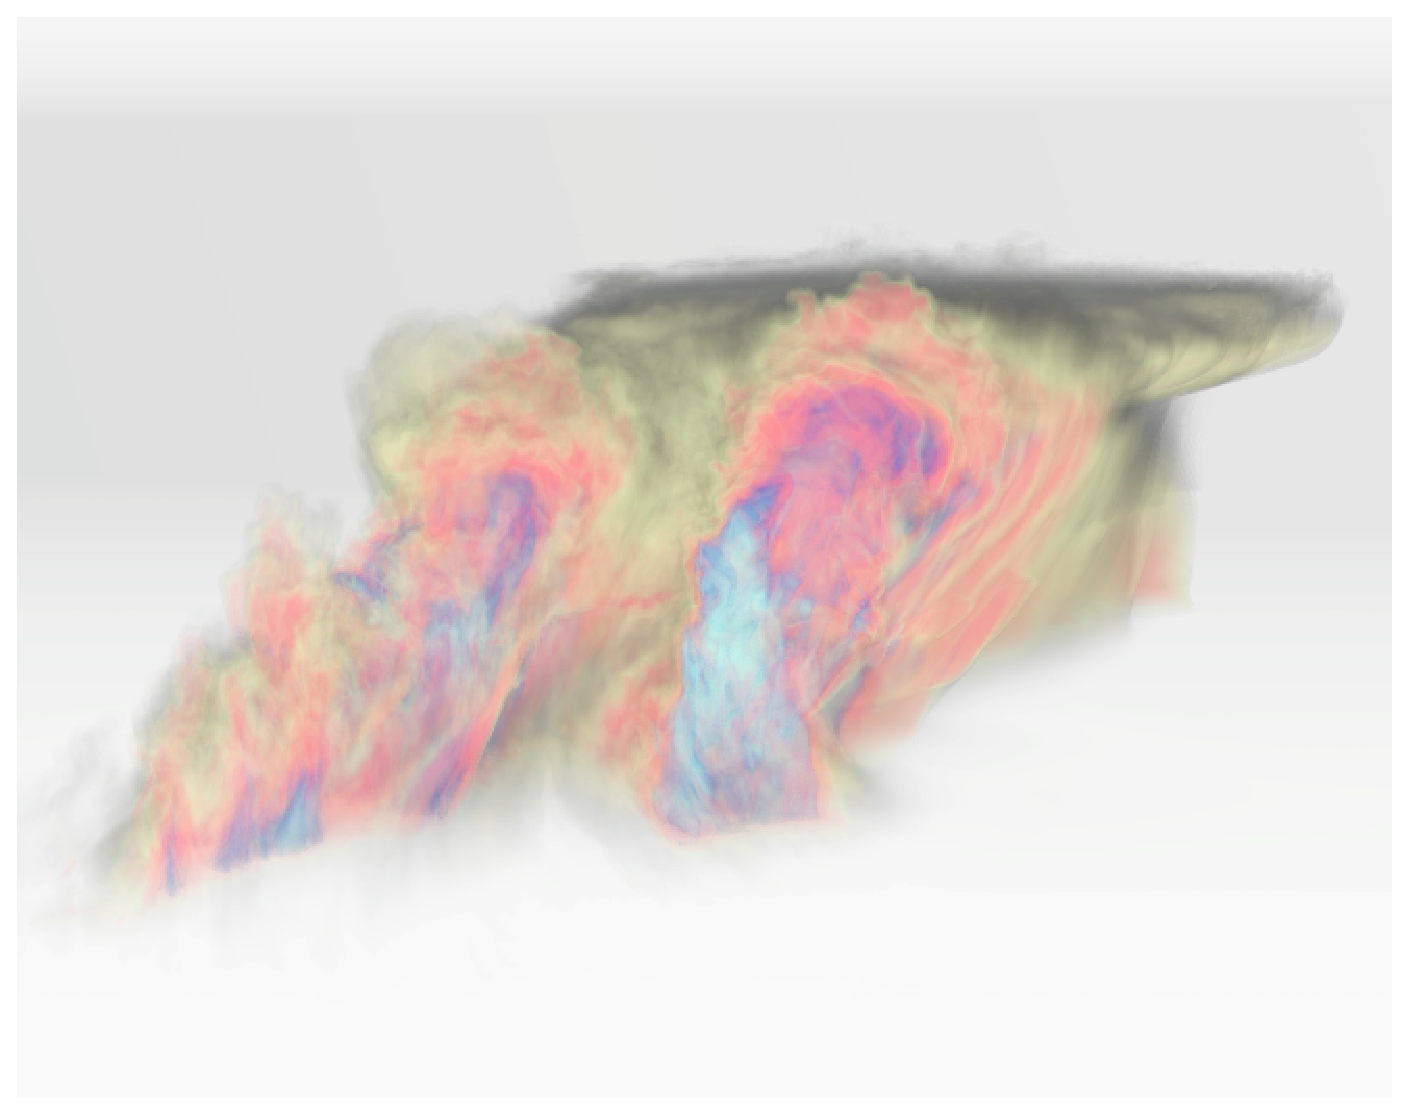
\includegraphics[width=5cm,height=5cm]{figures/cm1-raycasting.eps}}}
	\quad
	\subfigure[CM1 Isosurface]{
	\fbox{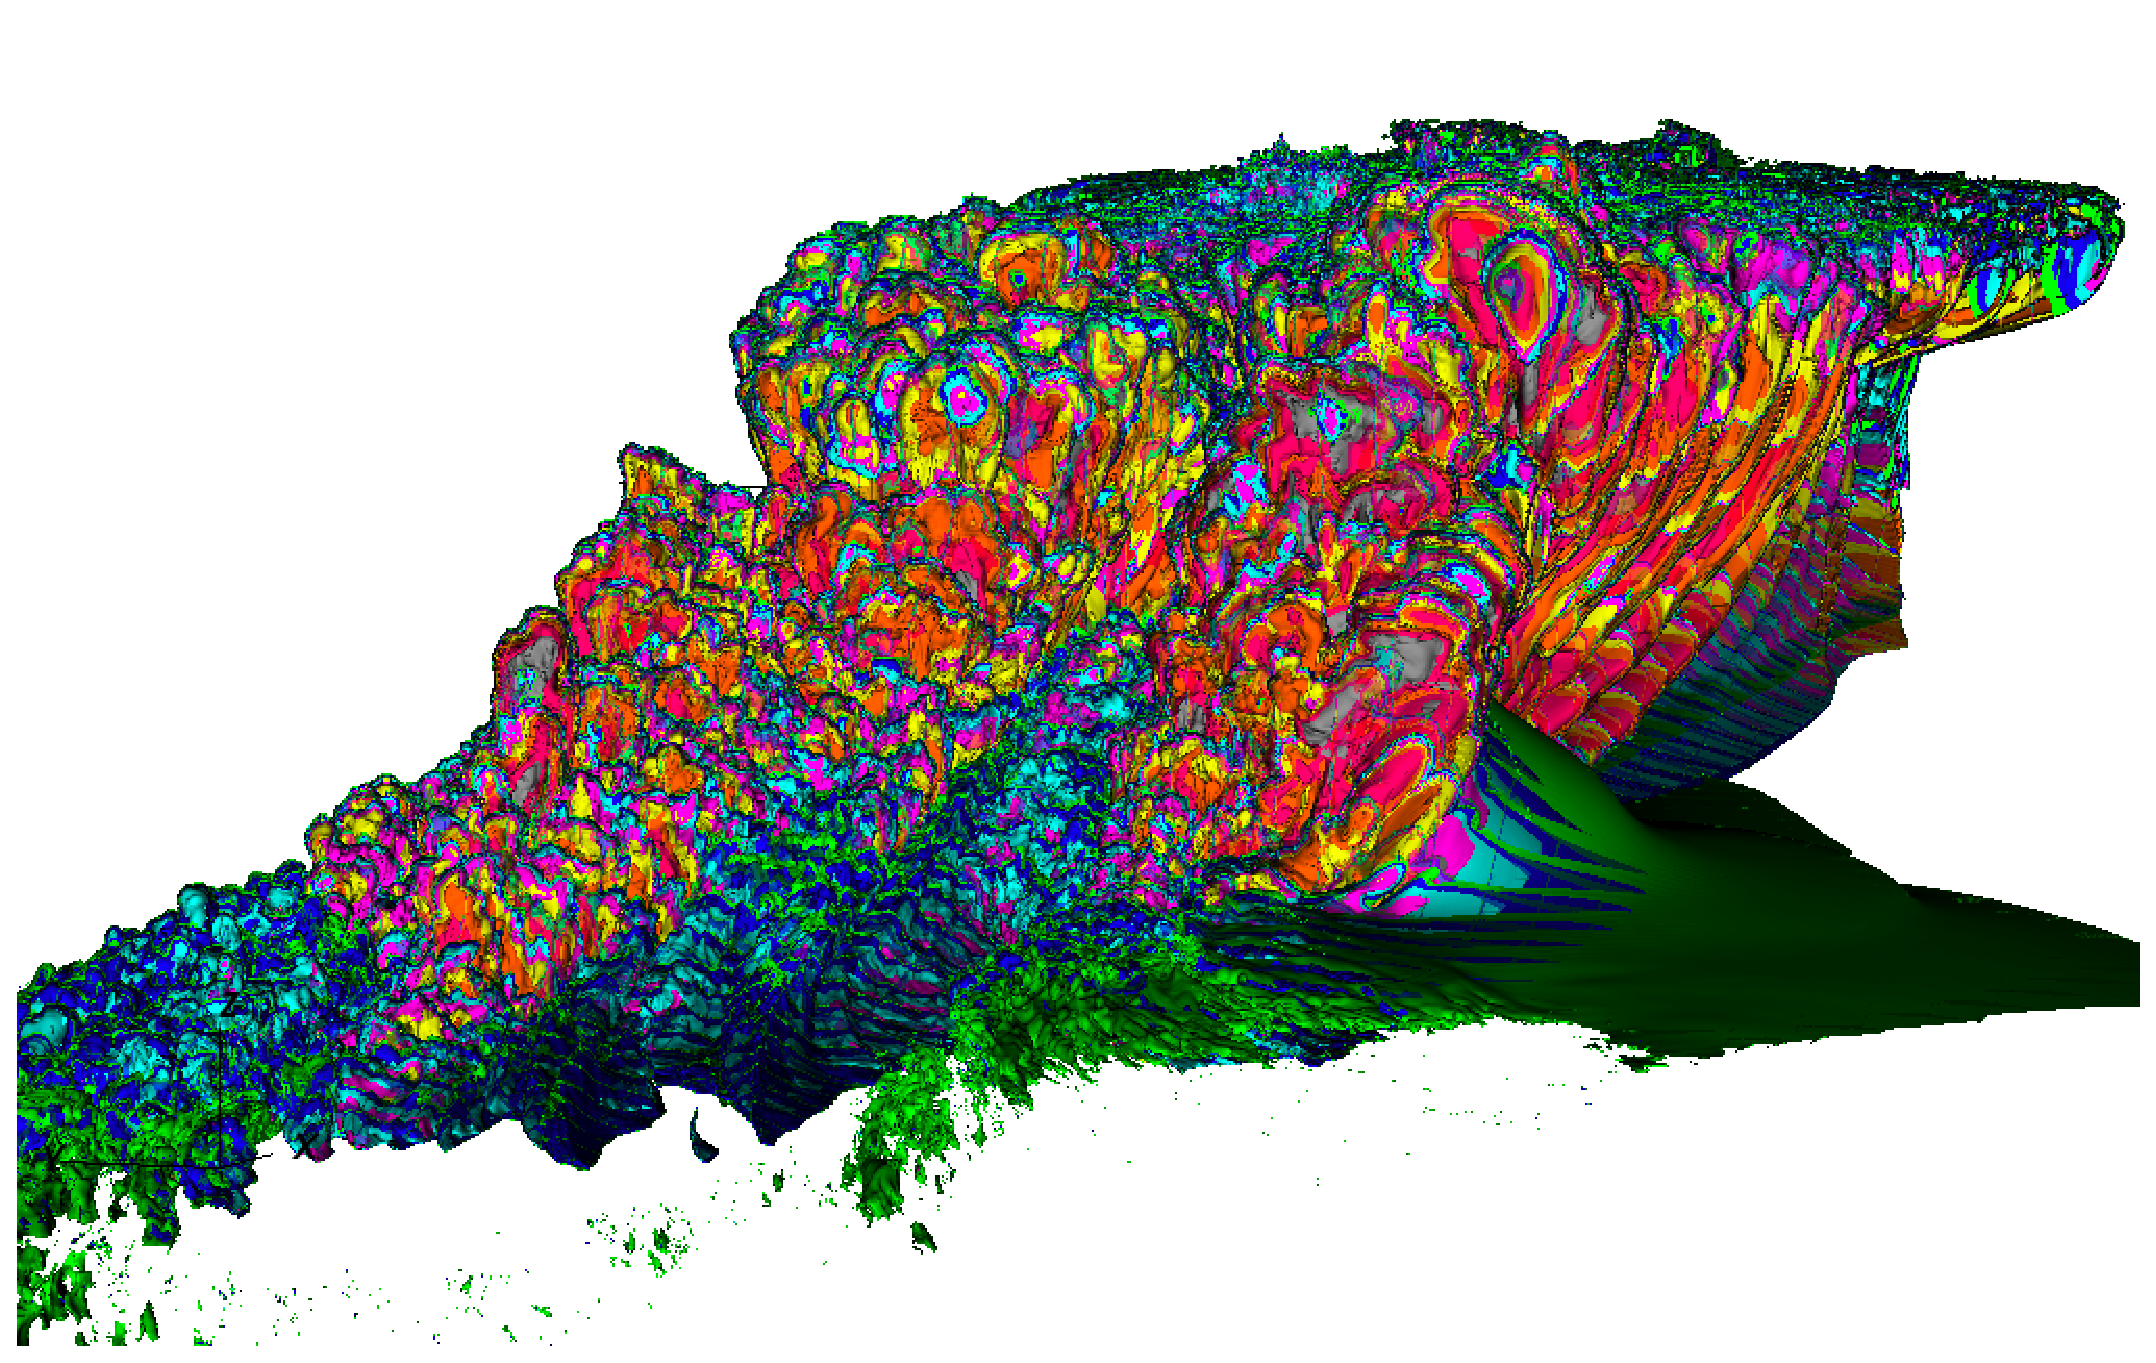
\includegraphics[width=5cm,height=5cm]{figures/cm1-isosurface.eps}}}
	
	\subfigure[CM1 Color Map]{
	\fbox{\includegraphics[width=5cm,height=5cm]{figures/cm1-dbz-colormap.eps}}}
	\quad
	\subfigure[Nek5000 Isosurface]{
	\fbox{\includegraphics[width=5cm,height=5cm]{figures/nek5-volume.eps}}}
	
	\caption[Example of visualizations from the CM1 and Nek5000 simulations]{Example results obtained in situ with Damaris:
	(a) Ray-casting of the \emph{dbz} variable on 6400 cores (Blue Waters).
	(b) 10-level isosurface of the DBZ variable on 6400 cores (Blue Waters).
	(c) Color map of the DBZ variable on 256 cores (Blue Waters).
	(d) Ten-level isosurface of the $y$ velocity field in 
	the TurbChannel configuration of Nek5000.}\label{fig:visualresults}
\end{figure}

The experiments were done on the Blue Waters supercomputer, NCSA's Cray XE6 
Petascale supercomputer~\cite{bluewaters}.
Our goal is to show that ISV approaches depend on the scalability of the rendering algorithm 
being used. We therefore complete a strong-scaling evaluation of two 
rendering methods described bellow.

\paragraph{Methodology}
CM1 requires a long run time before an interesting atmospheric phenomenon appears,
and such a phenomenon may not appear at small scale. Yet, we need visualizable
phenomena to appear in order to evaluate the performance of in situ visualization tasks.
Thus we first ran CM1 with the help of atmospheric
scientists to produce relevant data. We generated a representative dataset of 
$3840 \times 3840 \times 400$ points spanning several iterations.

We then extracted the I/O kernel 
from the CM1 code and built a program that replays its behavior at a given scale 
and with a given resolution by reloading, redistributing and interpolating the 
precomputed data.
The I/O kernel, identical to the I/O part of the simulation, calls Damaris
functions to transfer the data to Damaris. Damaris then performs in situ visualization, 
either in a time-partitioning manner or using dedicated cores.

\paragraph{Time Partitioning vs. Dedicated Cores: Results}
We measured the time to complete a rendering (average of 15 
iterations) using time partitioning and dedicated cores for each scenario. 
The comparative results are reported in Figure~\ref{fig:cm1vistime}.

\begin{figure}[t]
\centering
	\subfigure[In Situ Isosurface]{
	\includegraphics[width=5.5cm]{figures/cm1-in-situ-isosurface.eps}}
	\quad
	\subfigure[In Situ Ray Casting]{
	\includegraphics[width=5.5cm]{figures/cm1-in-situ-ray-casting.eps}}
	\caption[Rendering time of in situ ray-casting and isosurfaces of CM1]{Rendering time using ray-casting and isosurfaces, with 
	time-partitioning and dedicated cores with CM1. Note that the number of cores 
	represents the total number used for the experiments; using a dedicated cores 
	approach, 1/16 of this total number is effectively used for in situ visualization,
	which explains the overall higher rendering time with dedicated cores.}
	\label{fig:cm1vistime}
\end{figure}

The isosurface algorithm scales well with the number of cores 
using both in situ approaches. A time-partitioning approach would thus be 
appropriate if the user does not need to hide the run time impact of in situ 
visualization.
However, on 6400 cores, it takes as much time 
to complete the rendering as on 400 dedicated cores. In
terms of pure computational power, an approach based on dedicated cores is thus 16 
times more efficient.

The ray-casting algorithm on the other hand has a poorer scalability. After 
decreasing, the rendering time goes up again at a 6400-core scale, and it 
becomes about twice more efficient to use a reduced number of dedicated 
cores to complete this same rendering.

\paragraph{Discussion.} The choice of using dedicated cores versus a time-partitioning ISV approach 
depends on (1) the intended visualization scenario, (2) the scale of the experiments and 
(3) the intended frequency of visual output. Our experiments indeed show that at small scale,
the performance of rendering algorithms are good enough to be executed in a time-partitioning manner,
provided that the user is ready to increase the run time of his simulation. At large scale however,
it becomes more efficient to use dedicated cores, especially when using ray-casting,
where the observed rendering performance is substantially better when using a reduced number of
processes.

%%%%%%%%%%%%%%%%%%%%%%%%%%%%%%%%%%%%%%%%%%%%%%%%%%%
% NEK5
%%%%%%%%%%%%%%%%%%%%%%%%%%%%%%%%%%%%%%%%%%%%%%%%%%%

\paragraph{Experiments with the Nek5000 Simulation}
Our goal in this series of experiments is to show the impact of in situ visualization
tasks on the run-time variability of the simulation, and to show how dedicated cores
help alleviating this variability. We show in particular the effect of 
interactivity on this variability. We use the Nek5000 code for this purpose.
In addition to the MATiS configuration already used in Section~\ref{sec:expIO}, we
use the \emph{TurbChannel} configuration, which was designed to run on 32 to 64 cores,
in order to assess the impact of 
interactivity on run time with a time-partitioning approach and with dedicated cores. 
Figure~\ref{fig:visualresults}~(d) shows the result of a 10-level 
isosurface rendering of the fluid velocity along the $y$ axis, with the 
TurbChannel case. We use the MATiS configuration to show the scalability of our 
approach based on Damaris against a standard, time-partitioning approach.

\paragraph{Results with the TurbChannel Configuration}
Experiments were carried out on the Reims \emph{stremi} cluster of the French 
Grid'5000 testbed, which features 40 nodes (HP ProLiant DL165 G7) with 24 cores
per node, connected through a 1G Ethernet network.

To assess the impact of in situ visualization on the run time, we run 
TurbChannel on 48 cores using the two approaches: first we use a 
time-partitioning mode, in which all 48 cores are used by the simulation and 
synchronously perform ISV. Then we switch on one dedicated core per node,
leading to 46 cores being used by the simulation while 2 cores asynchronously run 
the ISV tasks.

In each case, we consider four scenarios: 
\begin{enumerate}
	\item The simulation runs without visualization;
	\item A user connects VisIt to the simulation but does not ask for any output;
	\item The user asks for isosurfaces of the velocity fields but does not interact with VisIt any further 
	(letting the Damaris/Viz update the output after each iteration);
	\item The user has heavy interactions with the simulations (for example rendering different variables, 
using different algorithms, zooming on particular domains, changing the 
resolution).
\end{enumerate}

Figure~\ref{fig:nek5variability} presents a trace of the duration of each
iteration during the four aforementioned scenarios using the two approaches.
Figure~\ref{fig:nek5variability}~(a) shows that ISV using 
a time-partitioning approach has a large impact on the 
simulation run time, even when no interaction is performed. The simple fact of connecting
VisIt without rendering anything forces the simulation to at least update metadata at each iteration,
which takes time.
Figure~\ref{fig:nek5variability}~(b) shows that ISV based on dedicated cores, 
on the other hand, is completely transparent from the point of view of the simulation.

\begin{figure}[t]
\centering
	\subfigure[Time-Partitioning]{
	\includegraphics[width=5.5cm]{figures/turbchannel-time-partitioning.eps}}
	\quad
	\subfigure[Space-Partitioning]{
	\includegraphics[width=5.5cm]{figures/turbchannel-space-partitioning.eps}}
	\caption[Run-time variability in CM1 due to ISV]{Variability 
	in run time induced by different scenarios of in situ 
	interactive visualization.}\label{fig:nek5variability}
\end{figure}

\paragraph{Results with the MATiS Configuration}
We ran the MATiS configuration on 816 cores. Each 
iteration takes approximately one minute and due to the important number of points 
that the mesh contains, it is difficult to perform interactive visualization. 
We therefore connect VisIt and simply query for a 3D pseudo-color plot of the $vx$ 
variable that is then continuously updated.
For the following results, the time-partitioning approach outputs one image every time step,
while dedicated cores adapted the output frequency to one image every 25 
time steps.

Figure~\ref{fig:matisruntime} reports the behavior of the application with and 
without visualization performed, and with and without dedicated cores. 
Corresponding statistics are presented in Table~\ref{tab:matisstats}.

\begin{figure}[t]
\centering
	\subfigure[Time Partitioning, Without Visualization]{
	\includegraphics[width=5.5cm]{figures/matis-tp-no-viz.eps}}
	\quad
	\subfigure[Time Partitioning, With Visualization]{
	\includegraphics[width=5.5cm]{figures/matis-tp-viz.eps}}
	\subfigure[Space Partitioning, Without Visualization]{
	\includegraphics[width=5.5cm]{figures/matis-sp-no-viz.eps}}
	\quad
	\subfigure[Space Partitioning, With Visualization]{
	\includegraphics[width=5.5cm]{figures/matis-sp-viz.eps}}
	\caption[Iteration time of Nek5000's MATiS configuration with and without ISV]{Iteration time 
	of the MATiS configuration without visualization 
	(left) and with visualization enabled (right).
	Top: with time partitioning, visualization time adds to the simulation time. 
	Bottom: With dedicated cores, visualization time entirely overlaps with simulation time.}\label{fig:matisruntime}
\end{figure}

\begin{table}
	\center
\caption[Average iteration time of Nek5000's MATiS configuration]{Average 
	iteration time of the Nek5000 MATiS configuration with a
   time-partitioning approach and with dedicated cores, with and without 
   visualization.}\label{tab:matisstats}
   \begin{tabular}{|l|l|c|c|}
   \hline
\textbf{Iteration Time} & & Average & Std. dev. \\
	\hline
\multirow{2}{*}{Time Partitioning} & w/o vis. & 75.07 sec  & 22,93 \\
	& with vis. & 205.21 sec & 57.15 \\
	\hline
\multirow{2}{*}{Space Partitioning} & w/o vis. & 67.76 sec & 20.09 \\
	& with vis. & 64.79 sec  & 20.44 \\
	\hline
   \end{tabular}
\end{table}

Time-partitioning visualization not only increases the average run time but 
also increases the standard deviation of this run time, making it more unpredictable.
On the other hand, the approach based on dedicated cores yields more consistent results.
One might expect dedicated cores to interfere with the
simulation as it performs intensive communications while the simulation runs. 
However, in practice we observe very little run time variation.

We also remark that decreasing the number of cores used by the simulation actually
decreases its run time. This is due to the fact that Nek5000 reaches its
limit of scalability. Yet due to its memory requirements, it is still necessary to run
it on this number of nodes. In other words, as reducing the number of cores per node
actually used by the simulation increases its performance, it further motivates the
use of these spare cores for extra tasks such as visualization.

Finally, while the  time-partitioning approach performs visualization at every 
time step here, dedicated cores have adapted the frequency of 
its output to 1 image every 25 time steps.
If a time-partitioning approach were to only output 1 image every 25 time steps 
(which corresponds to having only the $25^{th}$ iteration being impacted 
in Figure~\ref{fig:matisruntime} (b)), the completion time for 25 time steps 
would be 2007 seconds on average.
With dedicated cores, this takes 1620 seconds, that is, a 20\% speedup. 
Furthermore, since dedicated cores enable the visualization and 
simulation tasks to overlap, the total run time is unchanged with the addition of ISV.


\section{Discussion: Dedicated Cores vs. Dedicated Nodes}
\label{sec:discussion}
Two important questions can be asked about approaches like Damaris,
which propose to dedicate cores for data processing and I/O.

\begin{itemize}
\item How many dedicated cores should be used?
\item How does dedicating cores compares with dedicating nodes?
\end{itemize}

In this section we propose to answer these two questions through experiments with
the CM1 and Nek5000 simulations on Grid'5000.
We implemented in Damaris the option to use dedicated nodes instead of dedicated cores.
Some details of this implementation are given hereafter, before diving into our
experimental results.

We restrict our study to I/O. The choice of dedicating cores over dedicating nodes
for in situ visualization indeed depends on too many parameters (including the amount
of data involved, the simulation, the platform, and most importantly the visualization scenarios)
and deserves an entire study that we reserve for a future work.

\subsection{Dedicated Nodes in Damaris}

In order to compare dedicated cores with dedicated nodes, we either needed a state-of-the-art 
framework that provides dedicated nodes, such as DataSpace~\cite{dataspace}, or to 
implement dedicated nodes inside the Damaris framework. We chose the later because 
(1) our simulations are already instrumented with Damaris' API, allowing us to switch between
each approach without having to modify the simulation with another framework's API, and
(2) comparing the use of dedicated cores in Damaris with the use of dedicated nodes in
another framework would make it harder to distinguish performance benefits coming from
the approach (dedicated cores vs. dedicated nodes) from performance benefits
coming from specific optimizations of the framework itself.
This following section gives an overview of our implementation of dedicated nodes in Damaris.

\subsubsection{Implementation}

%\begin{figure*}[t]
%\centering
%	\subfigure[Writing with Dedicated Cores]{
%	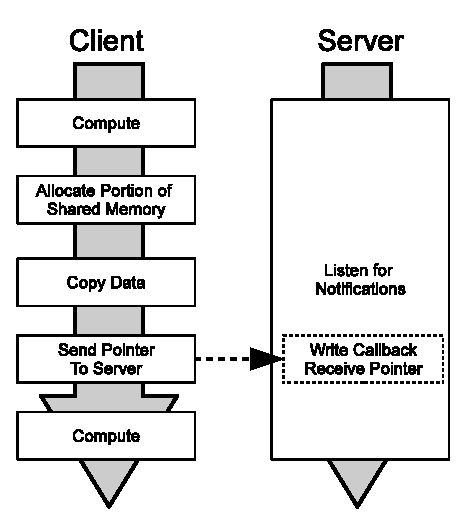
\includegraphics[width=7cm]{figures/damaris-comm-dc.eps}} 
%	\qquad
%	\subfigure[Writing with Dedicated Nodes]{
%	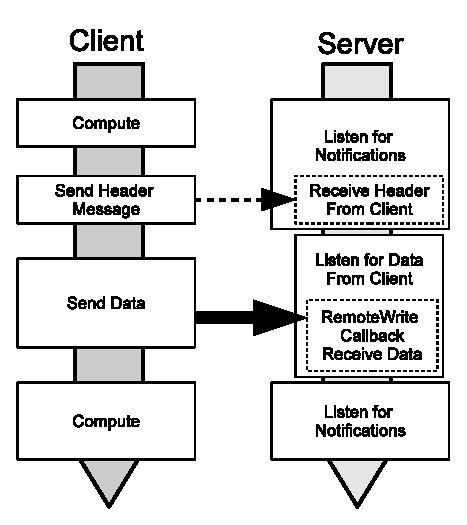
\includegraphics[width=7cm]{figures/damaris-comm-dn.eps}} 
%	%\quad
%	\subfigure[Legend]{
%	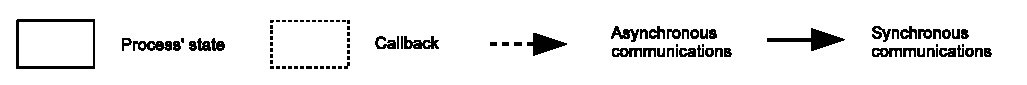
\includegraphics[width=14cm]{figures/energy/damaris-comm-legend.eps}} 
%	\caption[Data transfer protocols using dedicated cores and dedicated nodes]{Data transfer 
%	protocols using dedicated cores and dedicated nodes.}\label{fig:io:protocols}
%\end{figure*}

The implementation of dedicated nodes in Damaris relies on asynchronous MPI communications
through Damaris' Distributed Reactor.
Each simulation core is associated with a server
running in a dedicated node. A dedicated node hosts one server on each of its cores. 
Different simulation cores may thus interact with the same dedicated node, 
but with a different core (a different server) in this node.
%The protocol used to send data from the simulation to dedicated nodes is shown in Figure~\ref{fig:io:protocol-dn}.

When a client calls \texttt{damaris\_write}, it first
sends an event to its associated server. This event triggers a \texttt{RemoteWrite} callback
in the server. When the server enters this callback, it starts a blocking \texttt{receive} to
get the data sent by the client. The client sends its data
to the server, along with metadata information such as the \emph{id} of the variable to which the data belongs.
A buffer is maintained in clients to allow these transfers to be non-blocking. When the client
needs to send data to dedicated nodes, it copies the data into this buffer and issues a non-blocking \texttt{send}
to the server using the copied data (note that this communication phase is non-blocking in clients, but blocking
on servers). The status of this operation is checked in later calls to the 
Damaris API and the buffer is freed when the transfer is completed.

Other solutions exist in the literature, for example using RDMA~\cite{docan2010enabling}
(remote direct memory access). We chose to use simple asynchronous communications for simplicity
and portability. The flexibility of our design, along with the recent addition of 
dynamic RDMA windows in the MPI~3 standard, would ease such an RDMA-based implementation 
in Damaris in a near future.

\subsubsection{``Switching Gears''}

Switching between dedicated cores and dedicated nodes, as well as changing the number of
dedicated resources, can be done through the configuration, without recompiling the
application.

\begin{itemize}
\item \verb+<dedicated cores="n" nodes="0"/>+ enables $n$ dedicated cores per node.
The number of cores per node must divide evenly into the number of dedicated cores.
\item \verb+<dedicated cores="0" nodes="n"/>+ enables $n$ dedicated nodes. 
The total number of nodes must divide evenly into the number of dedicated nodes.
\item \verb+<dedicated cores="0" nodes="0"/>+ disables dedicated cores and nodes. It triggers the time-partitioning mode.
\end{itemize}

This configuration would allow for a hybrid approach that uses
both dedicated cores and dedicated nodes. However this approach is not supported by
Damaris yet, as we haven't found any real-life scenario that would benefit from it.

The implementation of all three approaches --time partitioning, dedicated cores, dedicated nodes-- 
within the same framework allows us to evaluate their respective performance in the next sections.

%%%%%%%%%%%%%%%%%%%%%%%%%%%%%%%%%%%%%%%%%%%%%%%%%%%%%%%%%%%%%%%%%%%%%%%%%%%%%%%%
%%%%%%%%%%%%%%%%%%%%%%%%%%%%%%%%%%%%%%%%%%%%%%%%%%%%%%%%%%%%%%%%%%%%%%%%%%%%%%%%
%%%%%%%%%%%%%%%%%%%%%%%%%%%%%%%%%%%%%%%%%%%%%%%%%%%%%%%%%%%%%%%%%%%%%%%%%%%%%%%%
%%%%%%%%%%%%%%%%%%%%%%%%%%%%%%%%%%%%%%%%%%%%%%%%%%%%%%%%%%%%%%%%%%%%%%%%%%%%%%%%

\subsection{Dedicated Core(s) vs. Dedicated Nodes: an Experimental Insight}

In the following, we present the results obtained with the Nek5000 and CM1 simulations,
using the different modes in which Damaris can now operate.

\subsubsection{Results with the Nek5000 Application}

We used the MATiS configuration of Nek5000 and ran it
on 30 nodes (720 cores) of the Grid'5000's \emph{stremi} cluster. We deploy
the OrangeFS parallel file system on 4 additional nodes of this cluster.
All nodes (including the file system) communicate through a 1G Ethernet network.

Nek5000 initially writes most of its checkpoint/restart data in the form of ASCII files, 
which appeared to be highly inefficient compared to using a high-level data format such as HDF5.
We thus rewrote its I/O part as an HDF5-based plugin for Damaris, and used Damaris
in 7 configurations: without dedicated resources  (time partitioning, abbreviated TP), 
using 1, 2, or 3 dedicated cores per node (abbreviated DC(1), DC(2) and DC(3)), 
and using 2, 3 or 5 dedicated nodes (DN(14:1), DN(9:1), DN(5:1) respectively, where the notation $x:y$ represents
the ratio of computation nodes, $x$, to dedicated nodes $y$). Despite the different number of
simulation cores in each configuration, the same mesh is used as input for Nek5000 and, 
therefore, the same amount of data is produced (about 3.5~GB per iteration).
We run Nek5000 for 10 such iterations in each configuration.

\begin{figure}
	\begin{center}
	\subfigure[Average iteration time]{
		\includegraphics[width=5.5cm]{figures/damaris-nek5-runtime-tpdcdn.eps}
	}\quad
	\subfigure[Average I/O time]{
		\includegraphics[width=5.5cm]{figures/damaris-nek5-io-time-tpdcdn.eps}
	}
	\caption{Experiment with Nek5000 on 720 cores of Grid'5000 \emph{stremi} cluster. 
	Damaris is configured to use either no dedicated resources (TP), $x = $1, 2 or 3 dedicated cores (DC($x$)),
	or a ratio of $x$ computation nodes to $y$ dedicated nodes (DN($x:y$)). 
	We report (a) the average, maximum and minimum time of a single 
	iteration (computation+I/O), and (b) the average, maximum and minimum time (logarithmic scale) 
	of an I/O phase from the point of view of the simulation.}\label{fig:nek5dcdn1}
	\end{center}
\end{figure}

\paragraph{Overall run time} All configurations based on dedicated resources enable a 40\% decrease of 
overall run time compared with the time-partitioning configuration. Note that because of the inherent 
variability of the duration of the computation phases within a single iteration (represented in 
Figure~\ref{fig:nek5dcdn1} (a) by the minimum and maximum iteration times), it is not possible to tell which of 
the configuration is actually the best one.
Considering these results only, we can argue that using more dedicated cores or more dedicated nodes is 
potentially an advantageous choice (as long as the efficiency of running your simulation is not affected) 
because it offers more resources for post-processing and I/O tasks.
The choice of using dedicated cores or dedicated nodes can then be based on the characteristics of these
post-processing time (scalability, memory requirement, execution time, etc.).

\paragraph{I/O impact}
Figure~\ref{fig:nek5dcdn1} (b) shows that the duration of the I/O phase as perceived by the simulation
becomes negligible when using an approach based on dedicated resources. Dedicated cores reduce this
time down to about 0.1 seconds, while dedicated nodes reduce it to about 0.04 seconds.
This difference in communication time between dedicated cores and dedicated nodes can be easily 
explained. When using dedicated cores, the client competes with other clients for the access to a 
mutex-protected segment of shared memory. When using dedicated
nodes on the other hand, this contention does not occur, as each client simply makes a local copy 
of its data and issues a non-blocking send that proceeds in parallel with the simulation. 
Therefore, while the I/O phase appears faster with dedicated nodes, our results do not show the potential
impact that background communications with dedicated nodes may have on the performance of the simulation.

\begin{figure}
	\begin{center}
	\subfigure[Average aggregate throughput]{
		\includegraphics[width=5.5cm]{figures/damaris-nek5-throughput-tpdcdn.eps}
	}\quad
	\subfigure[Spare time in dedicated resources]{
		\includegraphics[width=5.5cm]{figures/damaris-nek5-spare-tpdcdn.eps}
	}
	\caption{Experiment with Nek5000 on 720 cores of Grid'5000 \emph{stremi} cluster. 
	Damaris is configured to use either no dedicated resources (TP), $x = $1, 2 or 3 dedicated cores (DC($x$)),
	or a ratio of $x$ computation nodes to $y$ dedicated nodes (DN($x:y$)). 
	We report (a) the average, maximum and minimum aggregate throughput
	from writer processes, and (b) the spare time in dedicated processes for the approaches that leverage them.}\label{fig:nek5dcdn2}
	\end{center}
\end{figure}

\paragraph{Aggregate throughput}
From the point of view of writer processes (or from the point of view of the file system),
the different configurations lead to different aggregate throughput. Figure~\ref{fig:nek5dcdn2} (a) shows that
dedicated cores achieve the highest throughput. This throughput is slightly degraded as the number of
dedicated cores per node increases, due to contention between dedicated cores on the same node.
Dedicated nodes also increase the aggregate throughput compared with time partitioning, but do not achieve
the throughput of dedicated cores. This is due to the fact that all cores in dedicated nodes are writing,
and thus compete for the network access at the level of each single dedicated nodes.
Additionally, the lower throughput observed when using only two dedicated nodes can be explained
by the fact that the file system features four data servers. Therefore, dedicating only two nodes does not
fully take advantage of parallelism across writers.

\paragraph{Spare time}
Finally, Figure~\ref{fig:nek5dcdn2} (b) shows the spare time in dedicated resources. In all configurations
based on dedicated cores, the dedicated cores spend 10\% of their time writing, and remain idle 90\% of the time.
Dedicated nodes spend slightly more time writing (from 13 to 20\% of their time). This is a direct consequence
of the difference in aggregate throughput.

\paragraph{Conclusion}
Overall, all the configurations based on dedicated resources improve the simulation run time in a similar way.
These configurations however differ in other aspects. By avoiding contention at the level of a node, 
dedicated cores achieve a higher throughput and
therefore spare more time that can be used for data processing. Yet, if we weight this spare time
by the number of cores that can be used to leverage it (90 when dedicating 3 cores per node, 120 when
dedicating 5 nodes), the configuration based on 5 dedicated nodes appears to spare more resources (core-seconds)
in spite of sparing less time per core.

The choice of whether one should use an approach based on dedicated cores or dedicated nodes is of
course not restricted to these considerations. Some memory-bound simulations may not be able to afford 
allocating shared memory to dedicated cores, and would rather benefit from dedicated nodes. 
Some I/O intensive simulations on the other hand may not be able to transfer large amounts of data 
to a reduced number of dedicated nodes and will prefer dedicated cores.

\subsubsection{Results with the CM1 application}

In this section, we leverage experiments with the CM1 simulation to show that the choice of one 
approach over another also depends on the platform considered.

We used CM1 on Grid'5000's Nancy and Rennes sites.
On the Nancy site we use the \emph{graphene} cluster. Each node of this cluster consists of a 4-core
Intel Xeon 2.53~GHz CPU with 16~GB of RAM. Intra-cluster communication is done through a 1G Ethernet network.
A 20G InfiniBand network is used between these nodes and the OrangeFS file system deployed on 6 I/O servers.

On the Rennes site we use the \emph{parapluie} cluster, already presented in Section~\ref{sec:expIO}. 
The nodes communicate with one another through a 1G Ethernet network and with an OrangeFS file system
deployed on 3 servers across a 20G InfiniBand network.

We deploy CM1 on 32 nodes (128 cores) on the Nancy site. On the Rennes site, we deploy it on 16 nodes (384 cores).
In both cases, we configure CM1 to complete 2520 time steps. We vary its output frequency, using 10, 20 or 30 time steps
between each output. Damaris is configured to run with CM1 in five different scenarios that cover the three I/O approaches
considered: time partitioning, dedicated cores (one or two -- DC(1) and DC(2)), and dedicated
nodes using a ratio of 7:1 (DN(7:1), 7 compute nodes for one dedicated node) or 15:1 (DN(15:1), 15 compute nodes for one dedicated
node). DN(7:1) thus uses four dedicated nodes on the Nancy site, two on the Rennes site. DN(15:1) dedicates two nodes
on the Nancy site, one on the Rennes site.

\begin{figure}
	\begin{center}
	\subfigure[Run time of CM1 on Nancy cluster]{
		\includegraphics[width=5.5cm]{figures/nancy-cm1-runtime.eps}
	}\quad
	\subfigure[Run time of CM1 on Rennes cluster]{
		\includegraphics[width=5.5cm]{figures/rennes-cm1-runtime.eps}
	}
	\caption{Experiment with CM1 on Grid'5000 Rennes (24 cores per node) and Nancy (4 cores per node) sites. 
	Damaris is configured to use either no dedicated resources (TP), $x = $1 or 2 dedicated cores (DC($x$)),
	or a ratio of 7:1 or 15:1 dedicated nodes (DN(7:1) and DN(15:1)). We report total run time for 2520 time steps.}\label{fig:cm1dcdn}
	\end{center}
\end{figure}

\paragraph{Impact of the platform} Figure~\ref{fig:cm1dcdn} shows that in both clusters, dedicating resources drastically 
improve the performance of CM1 compared with a time-partitioning approach. 
Dedicating four nodes on Nancy enables an almost $3\times$ overall speedup, while
dedicating one core in each node on the Rennes cluster leads to more than $5\times$ speedup.
Our results also show that the best approach in terms of overall run time depends on the platform. It consists of 
using dedicated nodes with a 7:1 ratio on the Nancy cluster, and using one dedicated core per node on the Rennes cluster. 
This conclusion is not surprising, since the Nancy cluster only provides 4 cores per node. Dedicating some of these
cores thus has a large impact on the simulation. On the Rennes cluster, which provides 24 cores per node, dedicating
some of these cores does not remove such an important fraction of computational power from the simulation and is
thus more efficient than dedicating nodes.

\subsection{Conclusion}

Over the years, several research groups have proposed new approaches to I/O and data processing
based on dedicated resources. These approaches can be divided into a group of approaches based on dedicated
cores, and a group of approaches based on dedicated nodes. While Damaris was initially part of the first one,
we extended it to support a wider range of configurations. It now offers to dedicate either a subset of cores
in each multicore node, or entire nodes. Additionally, it also offers to not dedicate any resource at all,
performing all data processing and movement synchronously. This flexibility, made possible in particular
through a configuration file that allows us to switch between modes very easily, let us to compare these
approaches.

Our results show that dedicating resources for I/O is a highly efficient method to improve the I/O performance
of a simulation, both in terms of overall run time, aggregate throughput and performance variability. 
They also highlighted the fact that there is no clear advantage of one approach over the other: 
dedicating cores appears more efficient than dedicated nodes under certain conditions, and the opposite holds 
under different conditions. The choice
of one approach over the other may also depend on criteria other than the overall run time. Our experiments
with Nek5000 showed that while this run time is very similar under the different approaches, the resulting
aggregate throughput favors dedicating cores, while the resulting spared resources (spare time $\times$ number 
of cores in dedicated resources) advocates for using dedicated nodes. Our experiments with CM1 showed that
the choice of one approach over the other also depends on the platform. While an approach based on dedicated cores is
more suitable on a platform featuring a large number of cores per node, it may be more efficient to use dedicated nodes
on a platform with a reduced number of cores per node.


\section{Related Work}
\label{sec:related}
In this section, we position our work with respect to related work.
We start by discussing approaches that attempt at improving I/O performance.
We then examine approaches to in situ visualization.

\subsection{Damaris in the ``I/O Landscape''}

Through its capability of gathering data into larger buffers and files, 
Damaris can be compared to the data aggregation 
feature in ROMIO~\cite{thakur1999data}. This feature is an optimization of
Collective I/O that leverages a subset of processes, called ``aggregators'', to
actually perform the I/O on behalf of other processes.
Yet, data aggregation is performed synchronously in ROMIO:
all processes that do not perform actual writes in the file system must
wait for the aggregator processes to complete their operations. Besides,
aggregators are not dedicated processes, they run the simulation after completing their I/O.
Through dedicated cores, Damaris can perform data aggregation 
and potential transformations in an asynchronous
manner and still use the idle time remaining in the dedicated cores.

Other efforts focus on overlapping computation with I/O in order
to reduce the impact of I/O latency on overall performance. Overlap
techniques can be implemented directly within
simulations~\cite{patrick2008comparative}, using asynchronous
communications. Non-blocking I/O primitives started to appear as
part of the current MPI~3 standard, these primitives are still implemented as blocking in practice. 

Other approaches leverage data-staging and caching
mechanisms~\cite{nisar2009scaling,isaila2010design}, or
forwarding approaches~\cite{ali2009scalable} to achieve better I/O
performance. Forwarding architectures run on top of dedicated
resources in the platform, which are not configurable by the end-user, that is,
the user cannot run custom data processing in forwarding resources.
Similarly to the parallel file system, these dedicated resources are shared by all users. 
This leads to cross-application access contention and thus, to I/O variability. 
However, the trend toward I/O delegate systems underlines the need for new I/O approaches. 
Our approach relies on dedicated I/O cores at the
application level, or dedicated nodes bound to the application, 
rather than relying on hardware I/O-dedicated or forwarding
nodes, with the advantage of letting users configure their dedicated resources
to best fit their needs.

The use of local memory to alleviate the load on the file system is not new.
The Scalable Checkpoint/Restart (SRC) by Moody et al.~\cite{moody2010design} already makes
use of node-level storage to avoid the heavy load caused by periodic global 
checkpoints. Yet their work does not use dedicated resources or threads to 
handle or process data, and the checkpoints are not asynchronous.

\paragraph{Dedicated-Core-Based Approaches}
Closest to our work are the approaches by Li et al.~\cite{li2010functional},
and Ma et al.~\cite{ma2006highlevel}. While the
general goals of these approaches are similar (leveraging
service-dedicated cores for non-computational tasks), their design is
different, and so is the focus and the (much lower) scale of their
evaluation. The first one 
mainly explores the idea of using dedicated cores in conjunction with
SSDs to improve the overall I/O
throughput. Architecturally, it relies on a FUSE interface, which
introduces unnecessary copies through the kernel and reduces the degree of coupling 
between cores. Using small benchmarks we noticed that such a FUSE interface is 
about 10 times slower in transferring data between cores than using shared memory.
In the second, active buffers are handled by
dedicated processes that can run on any node and interact with cores
running the simulation through the network.  In contrast to both
approaches, Damaris makes a much more efficient design choice using
the shared intra-node memory, thereby avoiding costly copies and
buffering. The approach defended by Li et al. is
demonstrated on a small 32-node cluster (160 cores), where the maximum
scale used in the work by Ma et al. is 512~cores on a 
Power3 machine, for which the overall improvement achieved for the global
run time is marginal. Our experimental analysis is much more extensive
and more relevant for today's scales of HPC simulations: we
demonstrated the excellent scalability of Damaris on a real
supercomputer (Kraken, ranked $11^{th}$ in the Top500 supercomputer list at the time
of the experiments) with up to almost 10,000 cores, and with the CM1 tornado simulation, one of the
target applications of the Blue Waters post-Petascale supercomputer project. 
We demonstrated not only a speedup in I/O throughput by a
factor of 15 (never achieved by previous approaches), but we also
showed that Damaris totally hides the I/O jitter and substantially cuts
down the application run time at such high scales. With 
Damaris, the execution time for CM1 at this scale is even divided by 3.5 
compared to approaches based on collective I/O!  
Moreover, we further explored how
to leverage the spare time of the dedicated cores. We demonstrated for example
that it can be used to compress data by a factor of 6.

\subsection{Damaris in the ``In Situ Visualization Landscape''}

\paragraph{Loosely-Coupled Visualization Strategies}
Ellsworth et al.~\cite{ellsworth2006concurrent} propose to use distributed shared memory 
(DSM) to avoid writing files when performing concurrent visualization. Such an 
approach has the advantage of decoupling the simulation and visualization 
processes, but reading data from the memory of the simulation's processors can 
increase run time variability. The scalability
of a distributed shared memory design is also a limiting factor.

Rivi et al.~\cite{rivi2011insitu} introduce the ICARUS plugin for ParaView together with a 
description of VisIt and ParaView's in situ visualization interfaces. ICARUS employs an 
HDF5 DSM file driver to ship data to a distributed shared memory buffer that is
used as input to a ParaView pipeline. This DSM stores a view of the HDF5 
files that can be concurrently accessed by the simulation and visualization tools.
The HDF5 API allows to bridge the simulation and 
ParaView with minimum code changes (provided that the simulation already uses HDF5),
but it produces multiple copies of the data and a complete transformation of data
into an intermediate HDF5 representation.
Also, the visualization library on the remote resource requires the original data 
to conform to this HDF5 representation. Damaris, on the other hand, is not based
on any data format and efficiently leverages shared-memory to avoid as much as possible
unnecessary copies of data. Besides, its API is simpler than that of HDF5 for simulations
that do not already use HDF5.

Malakar et al.~\cite{malakar2010adaptive} present an adaptive framework for 
loosely-coupled visualization, in which data is sent over a network to a remote 
visualization cluster at a frequency that is dynamically adapted depending on resource availability. 
Our approach also adapts output frequency to resource usage.

The PreDatA~\cite{zheng2010predata} middleware proposes to dedicate a set of nodes as a 
staging area to perform a first step of data processing prior to I/O for the 
purpose of subsequent visualization. The coupling between the simulation and the
staging area is done through the ADIOS~\cite{lofstead2008flexible} I/O layer. 
The use of the ADIOS backend allows to decouple the simulation and the visualization by
simply integrating data analysis as part of an existing I/O stack~\cite{zheng2011highend}.
While Damaris borrows the use of an XML file from ADIOS in order to simplify its API,
it makes the orthogonal choice of using dedicated cores rather than dedicated nodes.
Thus it avoids potentially costly data movements across nodes.

GLEAN~\cite{rasquin2011electronic} provides in situ visualization capabilities with dedicated nodes. 
The authors use the PHASTA simulation on the Intrepid supercomputer 
and ParaView for analysis and visualization on the Eureka machine. 
Part of the analysis in GLEAN is done in a time-partitioning manner at the simulation side,
which makes it a hybrid approach involving tightly- 
and loosely-coupled in situ analysis. Our approach shares some of the same 
goals, namely to couple a simulation with run-time visualization, but we run the 
visualization tool on one core of the same node instead of dedicated nodes.
GLEAN is also used in conjunction with ADIOS~\cite{moreland2011examples}.

EPSN~\cite{esnard2006steering} is an environment providing steering and 
visualization capabilities to existing parallel simulations. Simulations 
instrumented with EPSN ship their data to a visualization pipeline running on a
remote cluster, thus EPSN is an hybrid approach including both code
changes and the use of additional remote resources. In contrast to EPSN, 
all visualization tasks using Damaris can be performed
on dedicated cores, closer to the simulation, thus reducing the network overhead.

Zheng et al.~\cite{zheng2011insitu} have provided a model to evaluate the tradeoff between 
in situ synchronous visualization and 
loosely-coupled visualization through staging areas. 
This model can be applied to compare in situ 
using dedicated cores instead of remote resources, with the 
difference being that approaches utilizing dedicated cores do not have network communication 
overhead.

\paragraph{Tightly-Coupled In Situ Visualization}
When it comes to tightly integrate analysis tasks in simulations codes, the 
existing solutions often do not meet all of the requirements presented in
Section~\ref{sec:background}.

SciRun~\cite{johnson1999interactive} is a complete computational-steering 
environment that includes visualization. Its in situ capabilities can be used 
with any simulation implemented with SciRun solvers and structures.
SciRun is an example of the trend towards integrating visualization, data 
analysis and computational steering in the simulation process.
Simulations are written specifically for use in SciRun in order to exchange 
data with zero data copy, but  
adapting an existing application to this framework can be a daunting task.

DIY~\cite{Peterka11Scalable} offers a number of communication primitives
allowing to easily build efficient parallel in situ analysis and visualization algorithms.
However it does not aim to provide a way to dedicate resources on which to run these algorithms.
DIY could therefor very well be coupled with Damaris to implement powerful in situ
analysis algorithms while Damaris provides the flexibility of running them on dedicated resources.

Tu et al.~\cite{tu2006mesh} propose an end-to-end approach for an earthquake 
simulation using the Hercule framework. All the components of the simulation, 
including visualization, run in parallel on the same machine, and the 
only output consists of a set of JPEG files.
The data processing tasks in Hercule are still performed in a synchronous manner, 
and any operation initiated by a process to perform these tasks impacts the 
performance of the simulation.

In the context of ADIOS, CoDS (Co-located DataSpaces)~\cite{zhang2012situ} 
builds a distributed object-based data space abstraction 
and can use dedicated nodes (and recently dedicated cores with shared memory) 
with PreDatA, DataStager and DataSpace. 
ADIOS+CoDS has also been used for code coupling~\cite{zhang2012ipdps} 
and demonstrated with different simulation models.
While the use of dedicated cores to accomplish two different tasks is a common
theme in our approach, our objective in this chapter was to compare the performance impact on the 
simulation of a collocated visualization task with a directly embedded 
visualization.
Besides, placement of data in shared memory in the aforementioned works is done through 
the ADIOS interface, which creates a copy of data from the simulation to the 
shared memory using a file-writing interface. We leverage the double-buffering 
technique usually implemented in simulations as an efficient alternative for sharing data.

Posteriorly to our work, Dreher and Rafin~\cite{dreher2014flexible} built on the FlowVR 
framework (initially proposed for real-time interactive parallel visualization in 
the context of virtual reality) to provide a solution integrating both time partitioning,
dedicated cores and dedicated nodes. They address usability
by providing a simple \emph{put}/\emph{get} interface and a Python script that describes
the various component of the visualization pipeline. They went one step further by
providing in situ interactive simulation steering in a cave-like system with haptic
devices~\cite{dreher2014fd169}, highlighting a case where the simulation process
and research are part of the same workflow.


\section{Conclusion and Future Directions}
\label{sec:conclusion}
As HPC resources exceeding millions of cores become a reality, science and engineering codes invariably
must be modified in order to efficiently exploit these resources. An important challenge in
maintaining high performance is data management, which nowadays does not only include writing
and storing data efficiently, but also analyzing and visualizing these data in order to retrieve a scientific insight.

This paper provides a comprehensive overview of Damaris, an approach which proposes to offload data management tasks,
including I/O, post-processing and visualization, into dedicated cores of multicore nodes. Damaris
efficiently leverages shared-memory to improve memory usage when transferring data from
cores running the simulation to cores running data-related tasks. Thanks to its plugin system and 
an external description of data, Damaris is highly adaptable to a wide range of simulations.

			We first used Damaris to offload I/O tasks in dedicated cores, and compared
			the resulting performance with the two standard approaches to I/O in HPC simulations:
			the File-per-process and the Collective I/O approaches. By gathering I/O operations
			in a reduced number of cores and by avoiding synchronization between these cores,
			Damaris is able to completely hide all I/O-related costs, and in particular the
			I/O variability. Our experiments using the CM1 atmospheric simulation and the Nek5000
			computation fluid dynamic, in particular on up to
			9216 cores of the Kraken supercomputer, showed that Damaris can achieve a 15 times
			higher throughput compared with the collective I/O approach. Damaris also dramatically
			reduces the application run time, leading to a $3.5\times$ speedup in CM1, for example.
			Observing that dedicated cores still remain idle a large fraction of the time,
			we implemented several improvements, including an overhead-free data compression
			that achieved up to 600\% compression ratio.
			
			We then leveraged the time spared by Damaris on dedicated cores by extending it 
			to support in situ visualization through a connection with the VisIt visualization software.
			We evaluated our Damaris-based in situ visualization framework on the Grid'5000 and Blue Waters platforms.
			We showed that Damaris can fully hide the performance variability induced 
			by in situ visualization tasks as well, even in scenarios involving interactions with a user. 
			Besides, Damaris reduces visualization-related code modifications 
			to a minimum in existing simulations.
			
			Finally we further extended Damaris to support the use of dedicated nodes instead
			of dedicated cores. Based on our framework, we perforùmed a thorough comparison
			of the dedicated cores, dedicated nodes and time-partitioning approaches for I/O
			on 3 different clusters of the Grid'5000 testbed, with the CM1 and Nek5000 simulations.
			Our evaluation shows that approaches based on dedicated resources always perform
			better than the time-partitioning approach for the selected simulations. They both manage
			to hide the I/O-related costs and, as a result, improve the overall simulation performance.
			While the choice of an approach based on dedicated cores over an approach based on
			dedicated nodes is primarily driven by the number of cores per node available in the 
			platform, this choice also depends on the scalability of the application, its memory usage,
			and the potential use of spare time in dedicated resources.
			
To our knowledge, Damaris is the first middleware available to the community\footnote{See \url{http://damaris.gforge.inria.fr}}  
that offers the use of dedicated cores or dedicated nodes to serve data management tasks ranging from
I/O to in situ visualization. This work paves the way for a number of new research directions with high potential impact. 
Our study of in situ visualization using Damaris and CM1 revealed that in some simulations
		such as climate models, an important fraction of the data produced by the simulation does not actually
		contain any part of the phenomenon that are of interest to scientists. When visualizing this data
		in situ, it thus becomes possible to lower the resolution of non-interesting parts in order
		to increase the performance of the visualization process, an approach that we call ``smart in situ visualization''.
		Challenges to implement smart in situ visualization include automatically discriminating relevant and non-relevant
		data within the simulation while this data is being produced. This detection should be made without
		user intervention and be fast enough to not diminish the overall performance of the visualization process.
		The plugin system of Damaris together with its existing connection with the VisIt visualization software 
		provide an excellent ground to implement and evaluate smart in situ visualization.
	
%
%In the future, we plan to leverage the high flexibility of Damaris to further improve
%the performance of in situ visualization by having Damaris automatically detect interesting features of the
%datasets produced by the simulation. 
We also plan to investigate ways to reduce the energy consumption  of simulations that use approaches like Damaris. We have already shown that the time spared by dedicated cores in Damaris can be leveraged to compress the data prior to storing it. An immediate question that can be asked is to which extent does compression in Damaris impacts this energy/performance tradeoff. On one hand, compression reduces the amount of data transferred and thus, the network traffic, which leads to lower energy consumption from data movements. On the other hand, compressing data requires more computation time and higher energy consumption as a result of data movement in the local memory hierarchy. Consequently, a promising direction will consist in investigating the tradeoff between energy, performance and compression level.


%% The Appendices part is started with the command \appendix;
%% appendix sections are then done as normal sections
%% \appendix

%% \section{}
%% \label{}

%% References
%%
%% Following citation commands can be used in the body text:
%% Usage of \cite is as follows:
%%   \cite{key}          ==>>  [#]
%%   \cite[chap. 2]{key} ==>>  [#, chap. 2]
%%   \citet{key}         ==>>  Author [#]

%% References with bibTeX database:

\bibliographystyle{model1-num-names}
\bibliography{biblio}

%% Authors are advised to submit their bibtex database files. They are
%% requested to list a bibtex style file in the manuscript if they do
%% not want to use model1-num-names.bst.

%% References without bibTeX database:

% \begin{thebibliography}{00}

%% \bibitem must have the following form:
%%   \bibitem{key}...
%%

% \bibitem{}

% \end{thebibliography}


\end{document}

%%
%% End of file `elsarticle-template-1-num.tex'.
